We performed experiments on the three datasets that correspond to a ``fair'' classification scenario and were previously used by~\cite{zemel2013learning}. In these datasets the ``nuisance'' or sensitive variable $\*s$ is significantly correlated with the label $\*y$ thus making the proper removal of $\*s$ challenging. Furthermore, we also experimented with the Amazon reviews dataset to make a connection with the ``domain-adaptation'' literature. Finally, we also experimented with a more general task on the extended Yale B dataset; that of learning invariant representations. 

\subsection{Datasets}
%\subsubsection{Fairness Datasets}
For the fairness task we experimented with three datasets that were previously used by~\citet{zemel2013learning}. The German dataset is the smallest one with $1000$ data points and the objective is to predict whether a person has a good or bad credit rating. The sensitive variable is the gender of the individual. The Adult income dataset contains $45,222$ entries and describes whether an account holder has over $\$50,000$ dollars in their account. The sensitive variable is age. Both of these are obtained from the UCI machine learning repository~\citep{UCI}. The health dataset is derived from the Heritage Health Prize\footnote{\url{www.heritagehealthprize.com}}. It is the largest of the three datasets with $147,473$ entries. The task is to predict whether a patient will spend any days in the hospital in the next year and the sensitive variable is the age of the individual. We use the same train/test/validation splits as~\citet{zemel2013learning} for our experiments. Finally we also binarized the data and used a multivariate Bernoulli distribution for $p_\theta(\*x_n|{\*z_1}_n,\*s_n) = \text{Bern}(\*x_n | \!\pi_n = \sigma(f_\theta({\*z_1}_n, \*s_n)))$, where $\sigma(\cdot)$ is the sigmoid function \footnote{$\sigma(t) = \frac{1}{1 + e^{-t}}$}.

%\subsection{Amazon Reviews Dataset}
For the domain adaptation task we used the Amazon reviews dataset (with similar preprocessing) that was also employed by~\citet{chen2012marginalized} and~\citet{2015arXiv150507818G}. It is composed from text reviews about particular products, where each product belongs to one out of four different domains: ``books'', ``dvd'', ``electronics'' and ``kitchen''. As a result we performed twelve domain adaptation tasks. The labels $\*y$ correspond to the sentiment of each review, i.e. either positive or negative. Since each feature vector $\*x$ is composed from counts of unigrams and bigrams we used a Poisson distribution for $p_\theta(\*x_n|{\*z_1}_n, \*s_n) = \text{Poisson}(\*x_n | \!\lambda_n = e^{f_\theta({\*z_1}_n, \*s_n)})$. It is also worthwhile to mention that we can fully exploit the semi-supervised nature of our model in this dataset, and thus for training we only use the source domain labels and consider the labels of the target domain as ``missing''.

%\subsection{Extended Yale B Dataset}
For the general task of learning invariant representations we used the Extended Yale B dataset, which was also employed in a similar fashion by~\citet{li2014learning}. It is composed from face images of 38 people under different lighting conditions (directions of the light source). Similarly to~\citet{li2014learning}, we created 5 states for the nuisance variable $\*s$: light source in upper right, lower right, lower left, upper left and the front. The labels $\*y$ correspond to the identity of the person. Following~\citet{li2014learning}, we used the same training, test set and no validation set. For the $p(\*x_n|{\*z_1}_n, \*s_n)$ distribution we used a Gaussian with means constrained in the 0-1 range (since we have intensity images) by a sigmoid, i.e. $p_\theta(\*x_n|{\*z_1}_n, \*s_n) = \mathcal{N}(\*x_n| \!\mu_n = \sigma(f_\theta({\*z_1}_n, \*s_n)), \!\sigma_n = e^{f_\theta({\*z_1}_n, \*s_n)})$.

\subsection{Experimental Setup}
For the Adult dataset both encoders, for $\*z_1$ and $\*z_2$, and both decoders, for $\*z_1$ and $\*x$, had one hidden layer of 100 units. For the Health dataset we had one hidden layer of 300 units for the $\*z_1$ encoder and $\*x$ decoder and one hidden layer of 150 units for the $\*z_2$ encoder and $\*z_1$ decoder. For the much smaller German dataset we used 60 hidden units for both encoders and decoders. Finally, for the Amazon reviews and Extended Yale B datasets we had one hidden layer with 500, 400 units respectively for the $\*z_1$ encoder, $\*x$ decoder, and 300, 100 units respectively for the $\*z_2$ encoder and $\*z_1$ decoder. On all of the datasets we used 50 latent dimensions for $\*z_1$ and $\*z_2$, except for the small German dataset, where we used 30 latent dimensions for both variables. For the predictive posterior $q_\phi(\*y|\*z_1)$ we used a simple Logistic regression classifier. Optimization of the objective function was done with Adam~\citep{DBLP:journals/corr/KingmaB14} using the default values for the hyperparameters, minibatches of 100 data points and temporal averaging. The MMD penalty was simply multiplied by the minibatch size so as to keep the scale of the penalty similar to the lower bound. Furthermore, the extra strength of the MMD, $\beta$, was tuned according to a validation set. The scaling of the supervised cost was low ($\alpha = 1 $) for the Adult, Health and German datasets due to the correlation of $\*s$ with $\*y$. On the Amazon reviews and Extended Yale B datasets however the scaling of the supervised cost was higher: $\alpha = 100 \cdot \frac{N_{\text{batch\_source}} + N_{\text{batch\_target}}}{N_{\text{batch\_source}}}$ for the Amazon reviews dataset (empirically determined after observing the classification loss on the first few iterations on the first source-target pair) and $\alpha = 200$ for the Extended Yale B dataset. Similarly, the scaling of the MMD penalty was $\beta = 100 \cdot N_{\text{batch}}$ for the Amazon reviews dataset and $\beta = 200 \cdot N_{\text{batch}}$ for the Extended Yale B.

Our evaluation is geared towards two fronts; removing information about $\*s$ and classification accuracy for $\*y$. To measure the information about $\*s$ in our new representation we simply train a classifier to predict $\*s$ from $\*z_1$. We utilize both Logistic Regression (LR) which is a simple linear classifier, and Random Forest (RF) which is a powerful non-linear classifier. Since on the datasets that we experimented with the nuisance variable $\*s$ is binary we can easily find the random chance accuracy for $\*s$ and measure the discriminatory information of $\*s$ in $\*z_1$. Furthermore, we also used the discrimination metric from~\cite{zemel2013learning} as well a  more ``informed'' version of the discrimination metric that instead of the predictions, takes into account the probabilities of the correct class. They are provided in the appendix A. Finally, for the classification performance on $\*y$ we used the predictive posterior $q_\phi(\*y|\*z_1)$ for the VAE/VFAE and a simple Logistic Regression for the original representations $\*x$. It should be noted that for the VFAE and VAE models we use a sample from $q_\phi(\*z_1|\*x, \*s)$ to make predictions, instead of using the mean. We found that the extra noise helps with invariance. 

We implemented the Learning Fair Representations~\citep{zemel2013learning} method (LFR) as a baseline using $K=50$ dimensions for the latent space. To measure the accuracy on $\*y$ in the results below we similarly used the LFR model predictions.

\subsection{Results}
\subsubsection{Fair classification}
The results for all three datasets can be seen in Figure~\ref{tab:fair_results}. Since we are dealing with the ``fair'' classification scenario here, low accuracy and discrimination against $\*s$ is more important than the accuracy on $\*y$ (as long as we do not produce degenerate representations).

\begin{figure}[ht]
   \centering
   \begin{subfigure}{\linewidth}
  \begin{subfigure}{.329\textwidth}
    \centering
        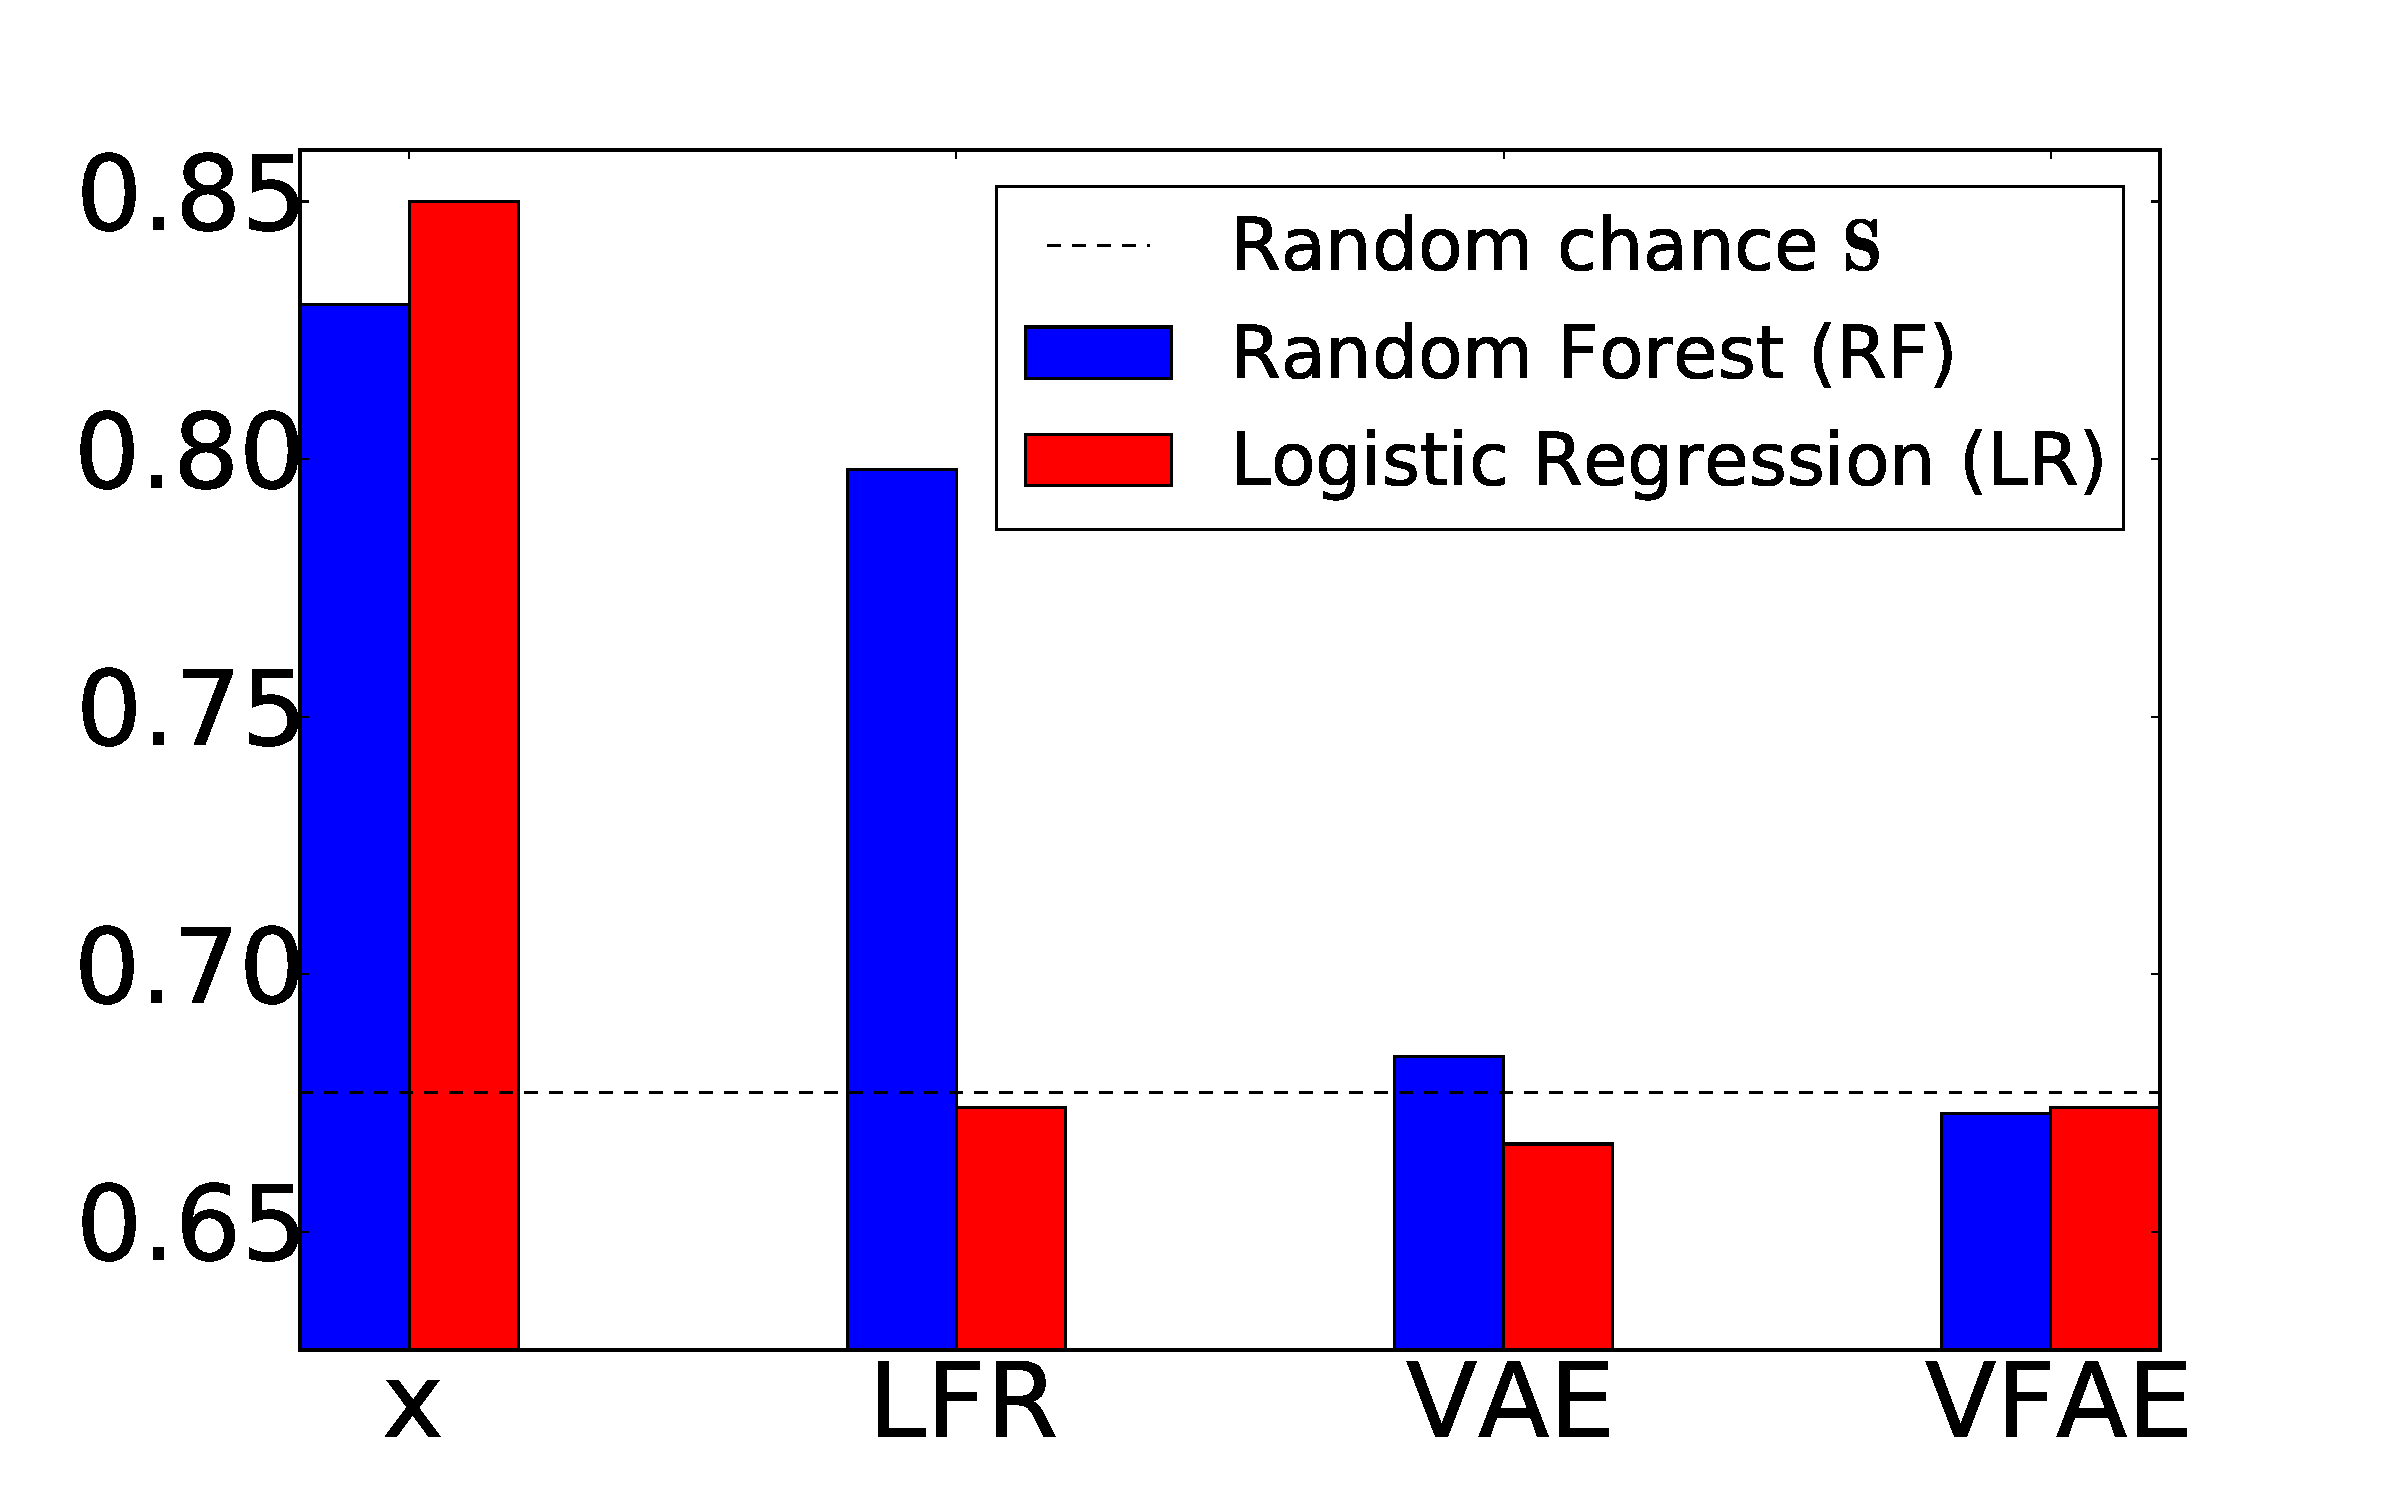
\includegraphics[width=1.1\linewidth]{adult_s.pdf}
  \end{subfigure} %
  \begin{subfigure}{.329\textwidth}
    \centering
        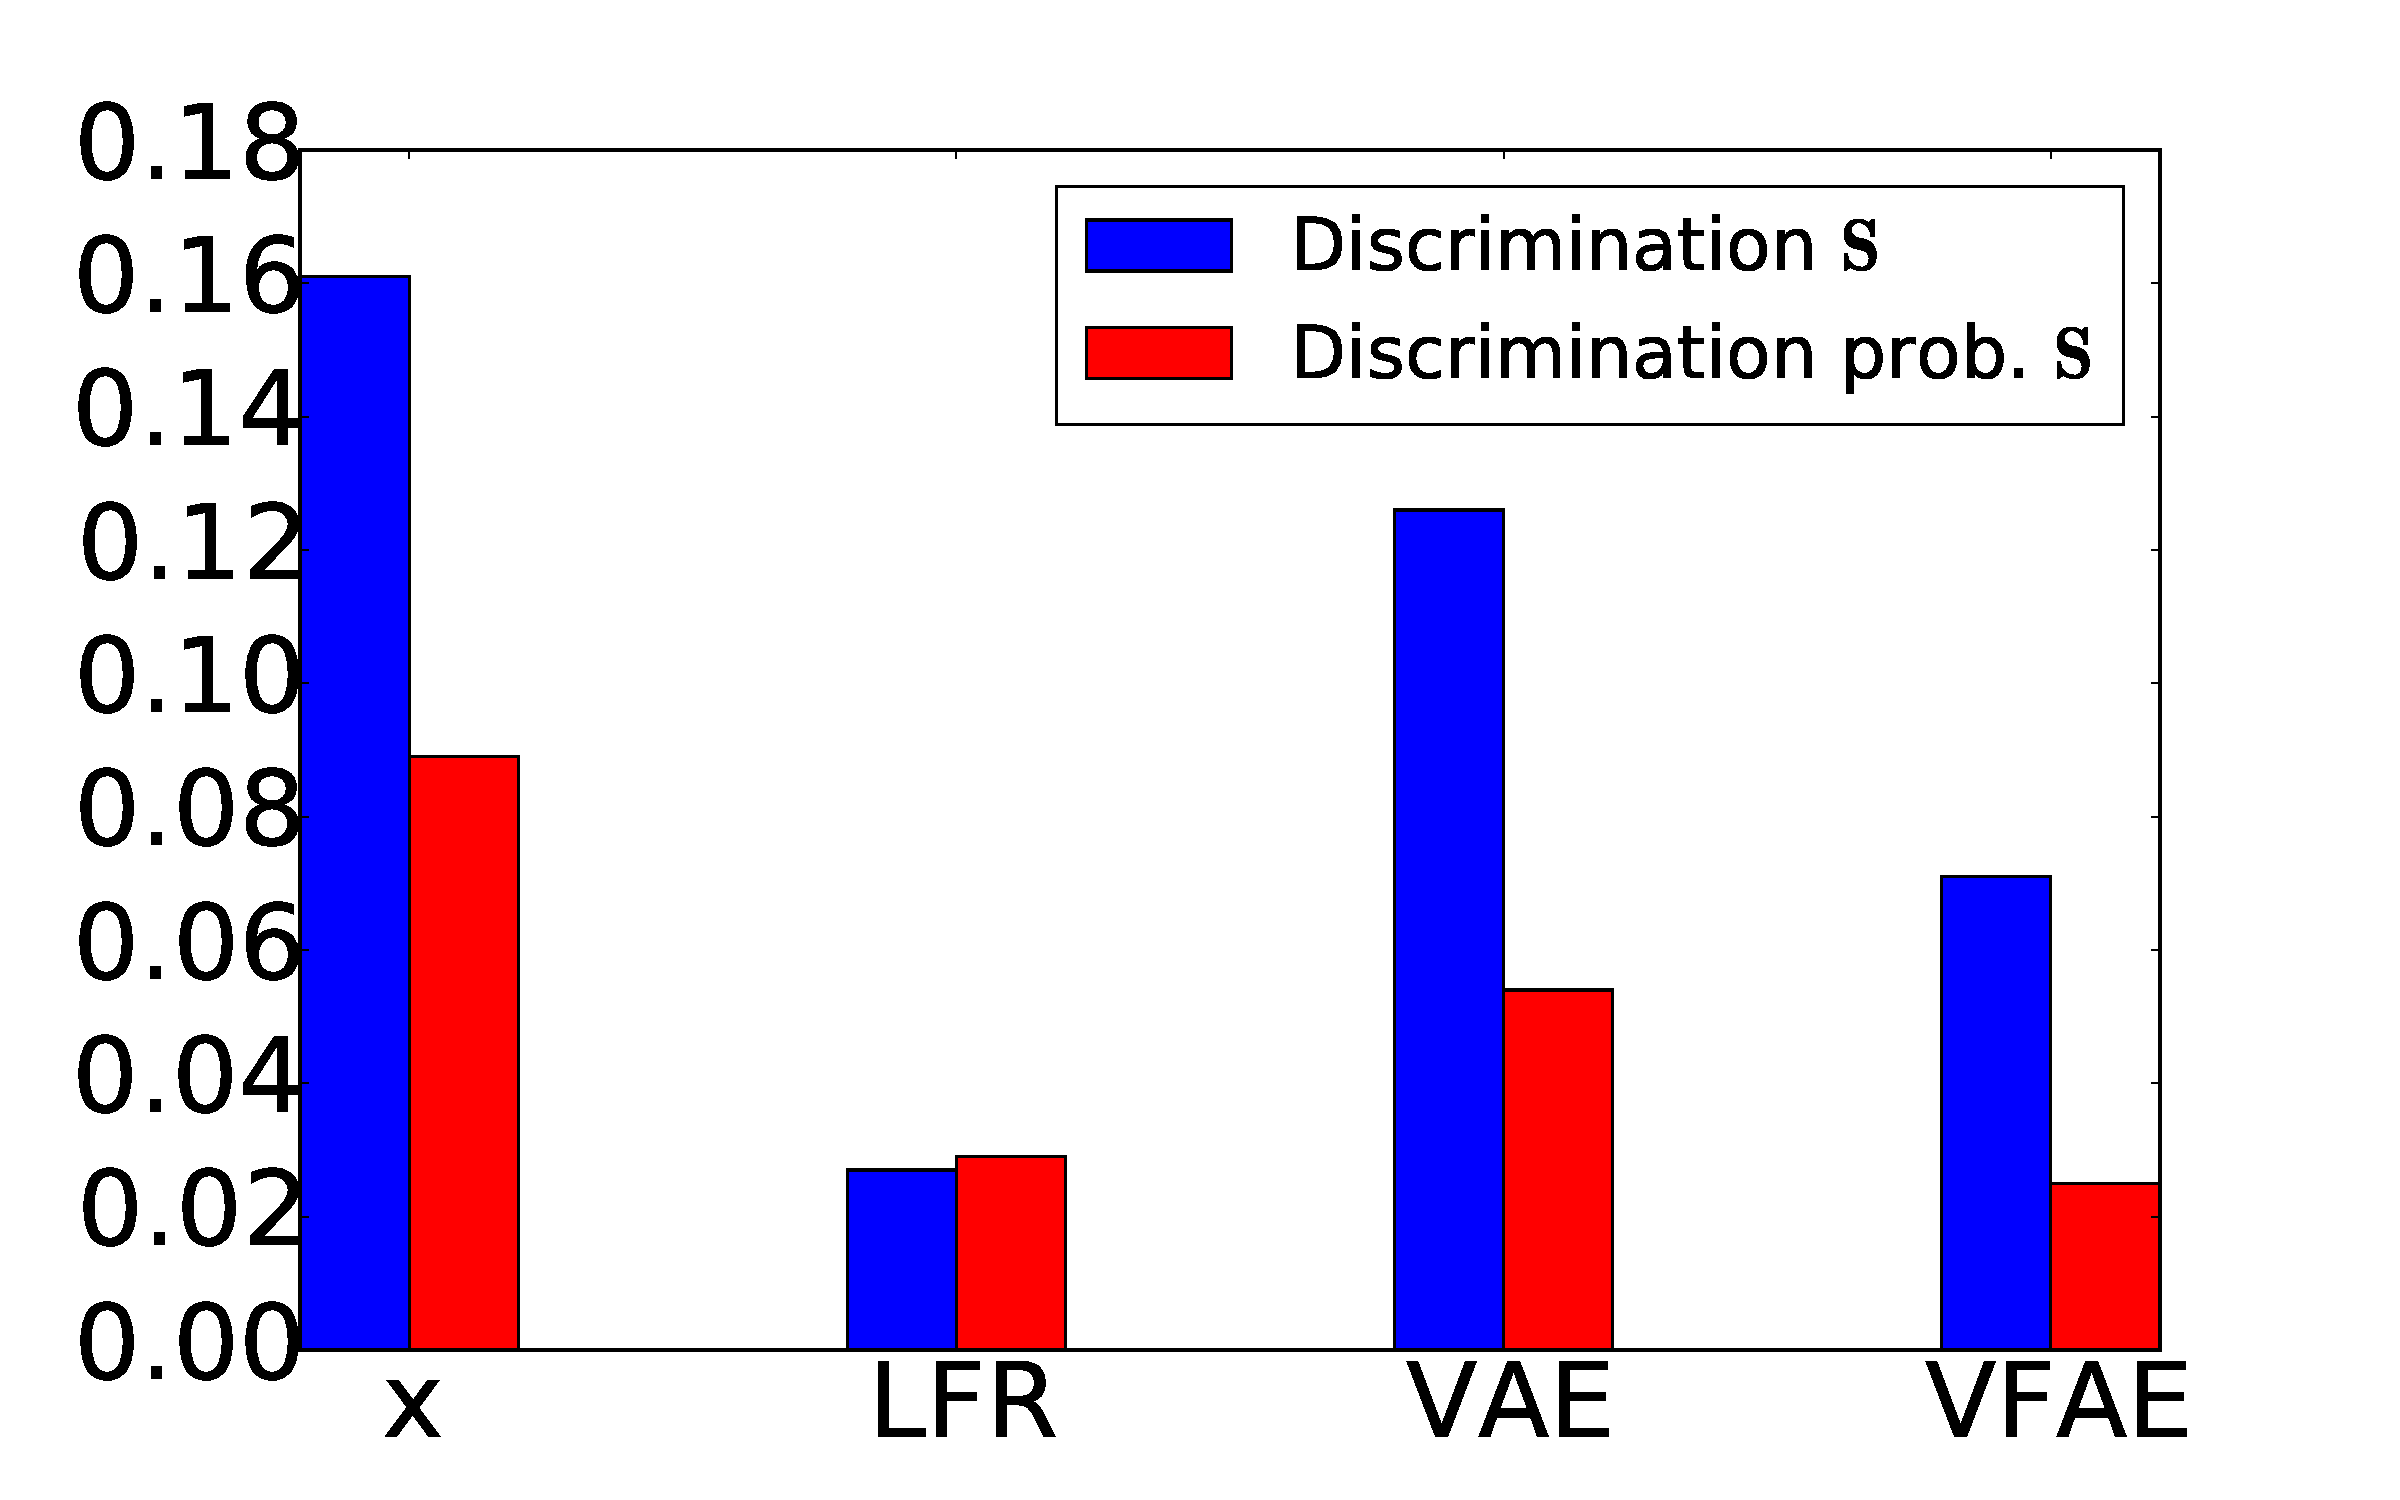
\includegraphics[width=1.1\linewidth]{adult_discr.pdf}
  \end{subfigure} %
  \begin{subfigure}{.329\textwidth}
    \centering
        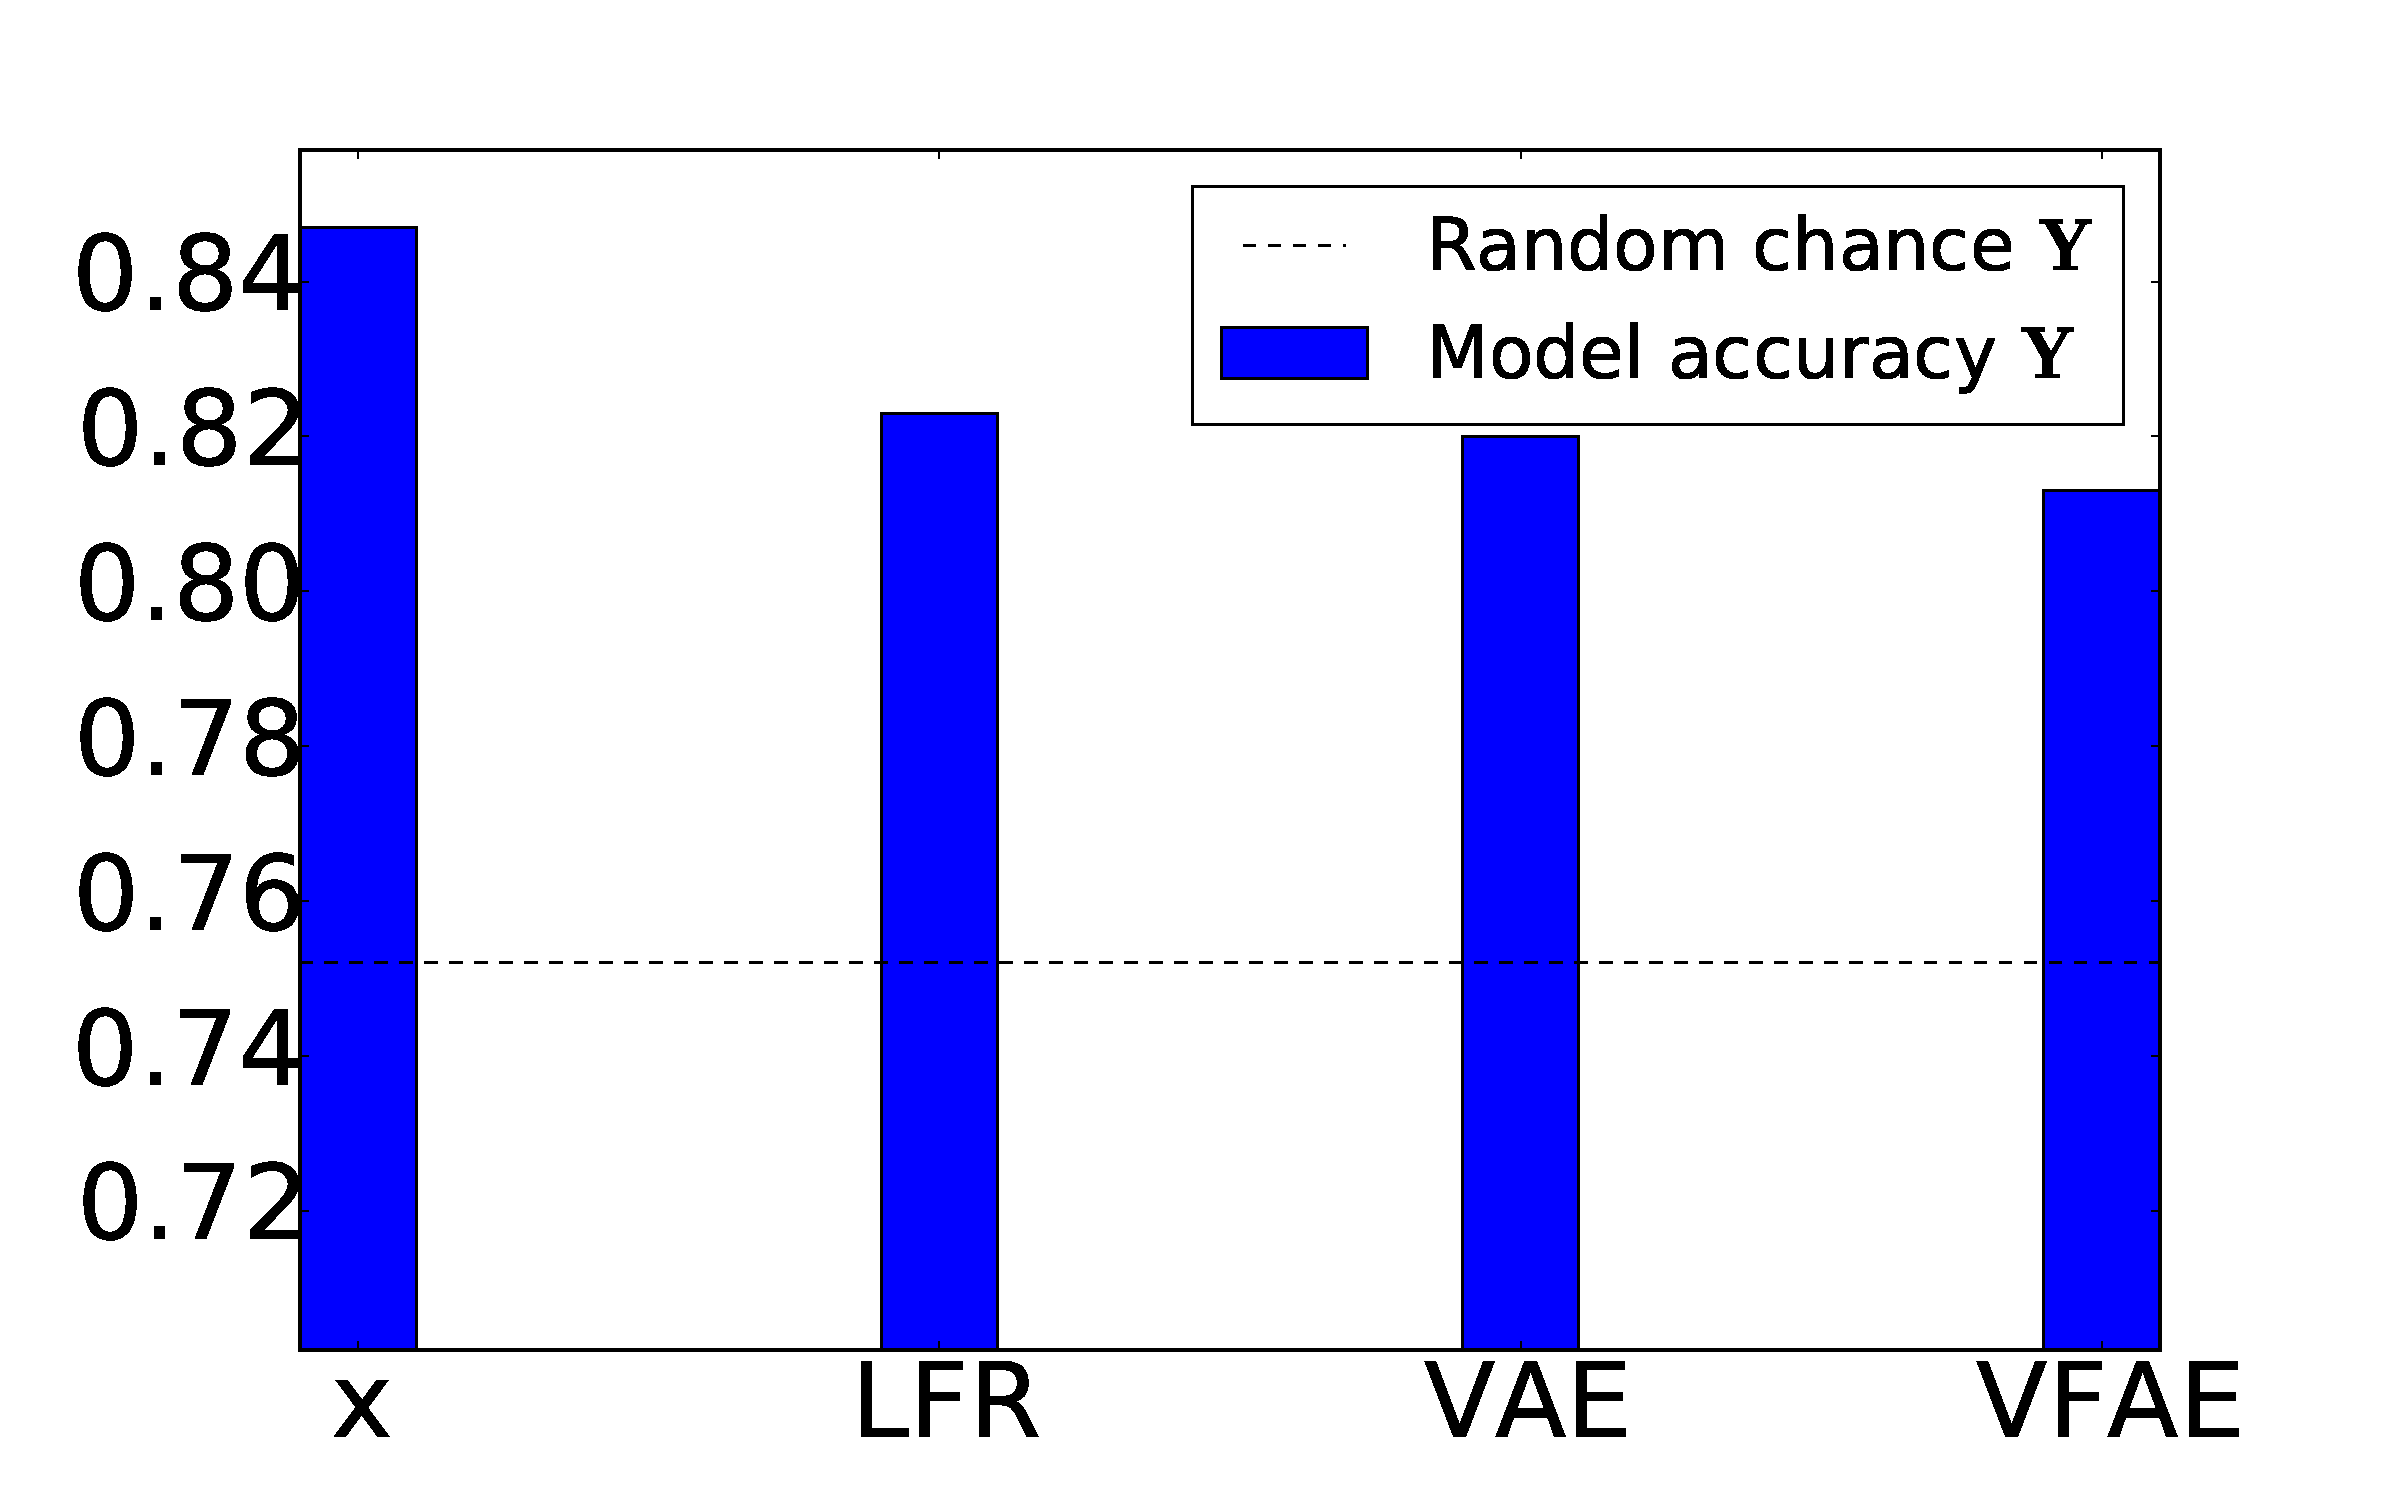
\includegraphics[width=1.1\linewidth]{adult_y.pdf}
  \end{subfigure}
  \caption{Adult dataset}
  \end{subfigure} \\
  \begin{subfigure}{\linewidth}
  \begin{subfigure}{.329\textwidth}
    \centering
        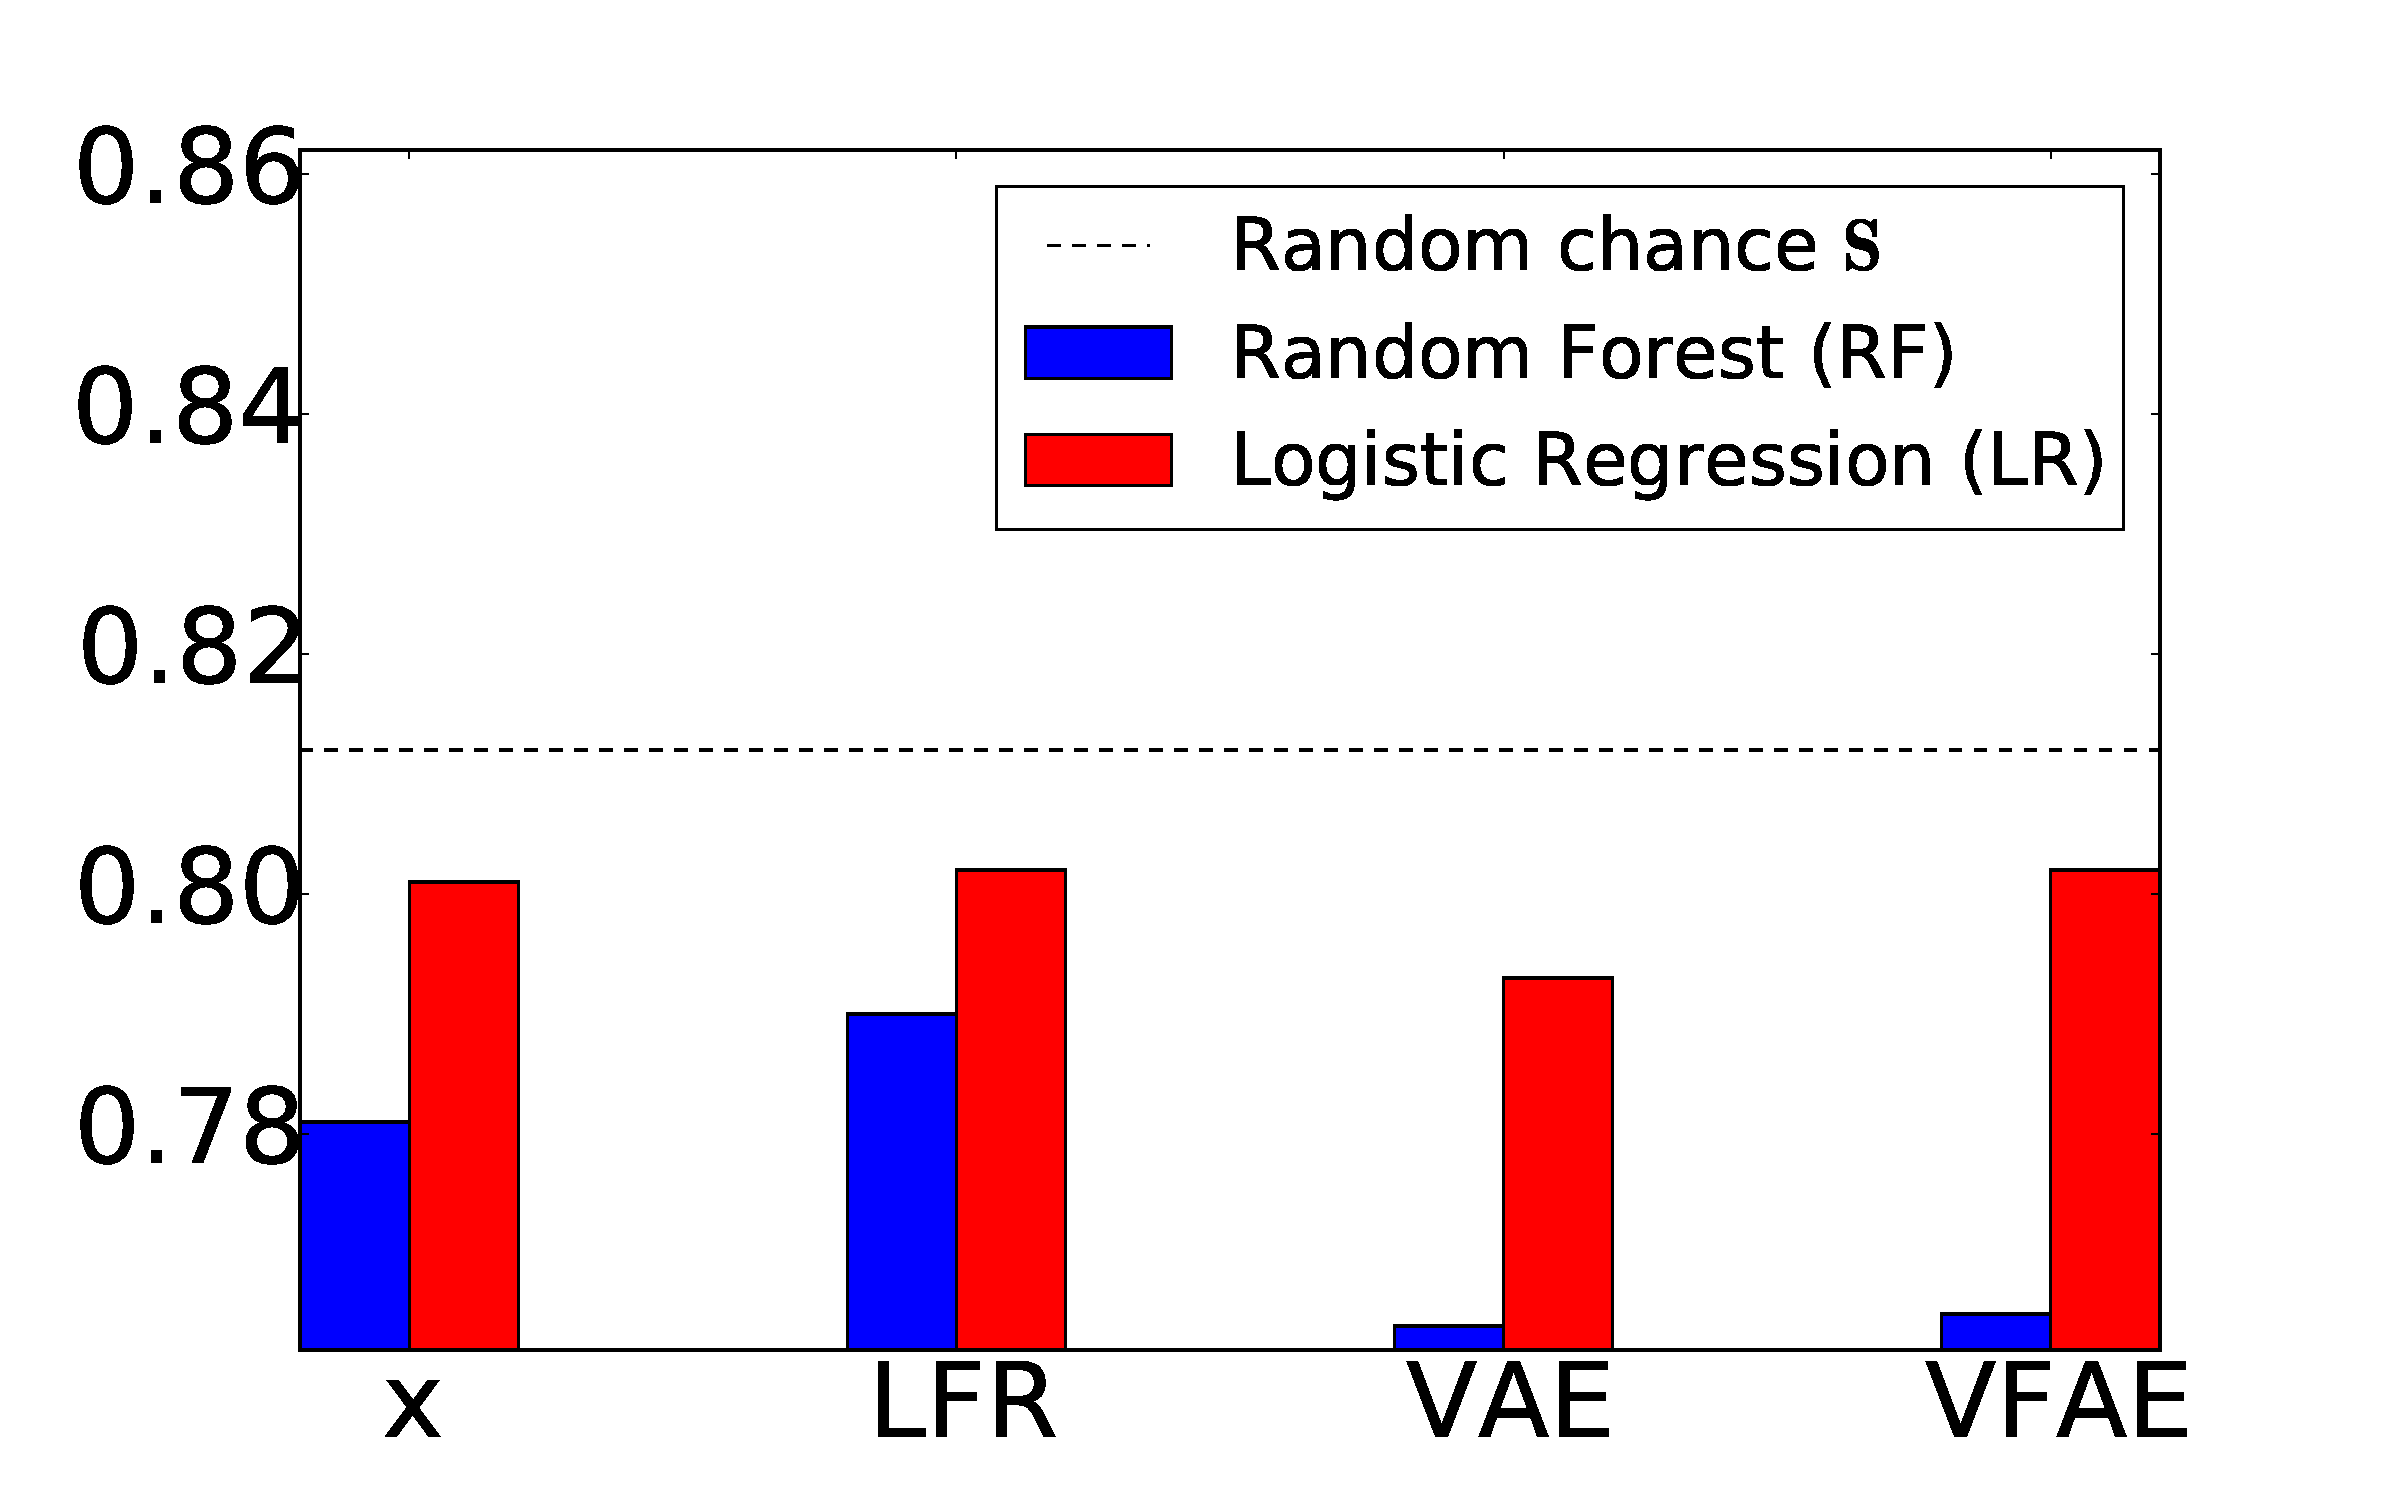
\includegraphics[width=1.1\linewidth]{german_s.pdf}
  \end{subfigure}%
    \begin{subfigure}{.329\textwidth}
    \centering
        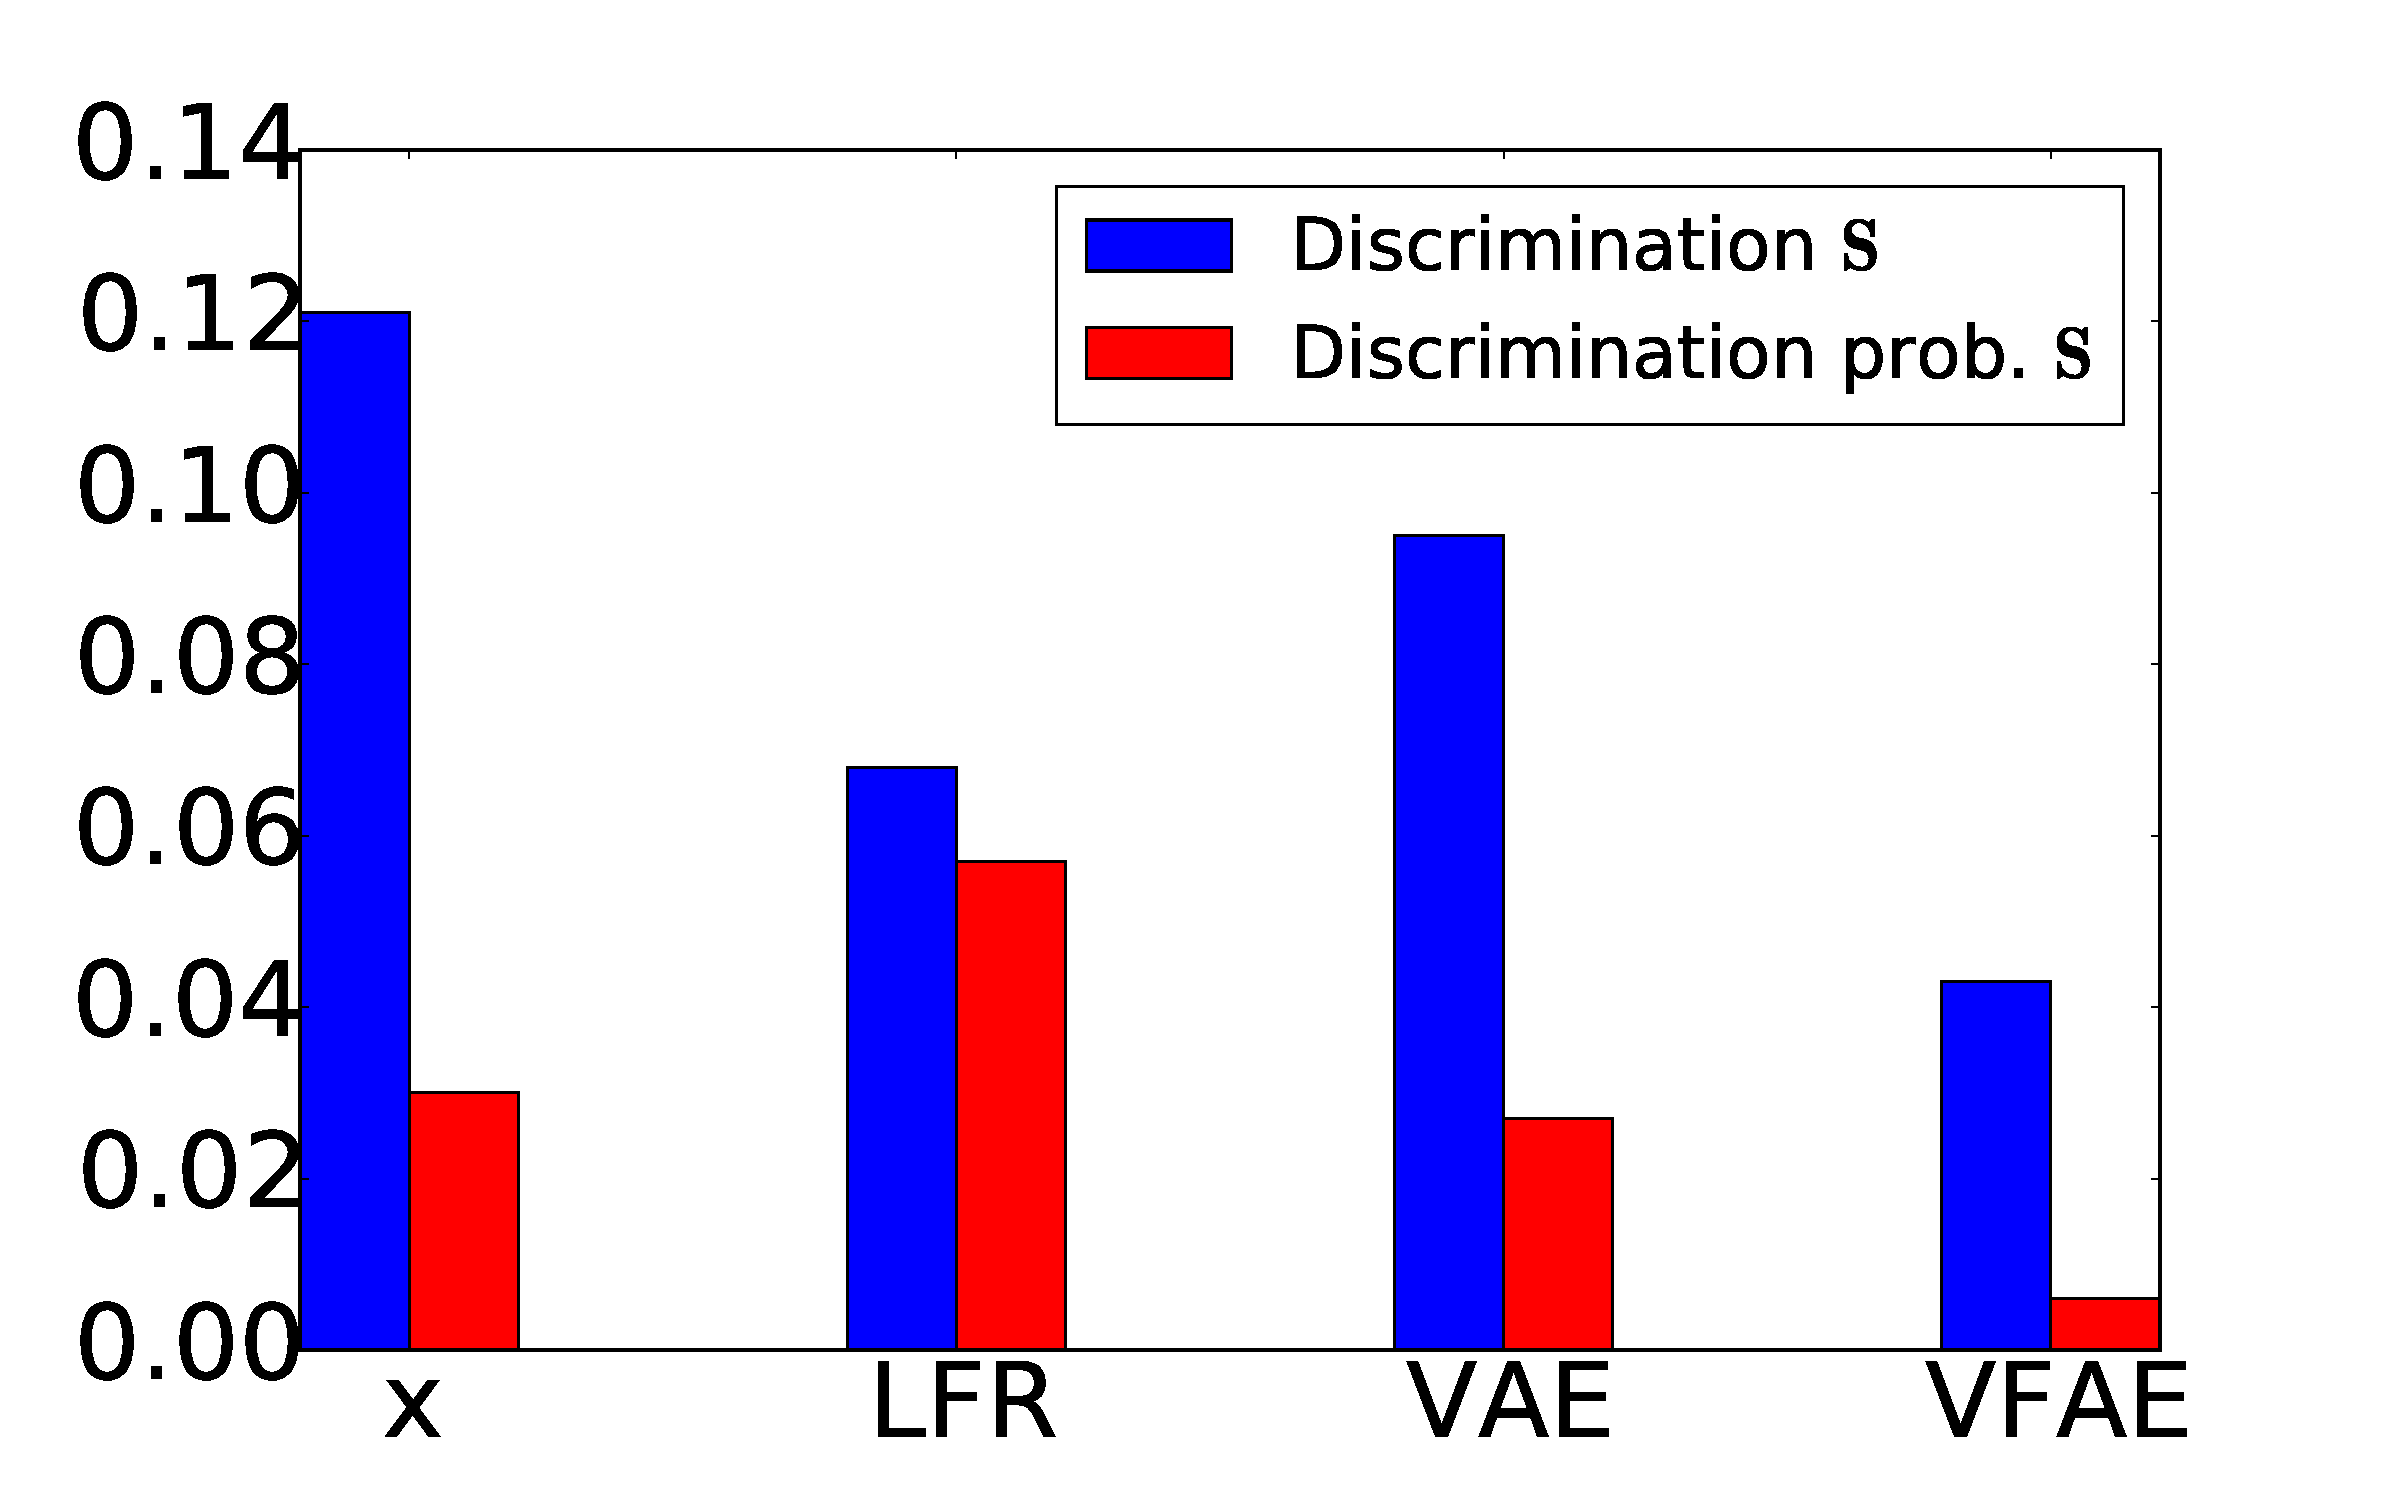
\includegraphics[width=1.1\linewidth]{german_discr.pdf}
  \end{subfigure}%
  \begin{subfigure}{.329\textwidth}
    \centering
        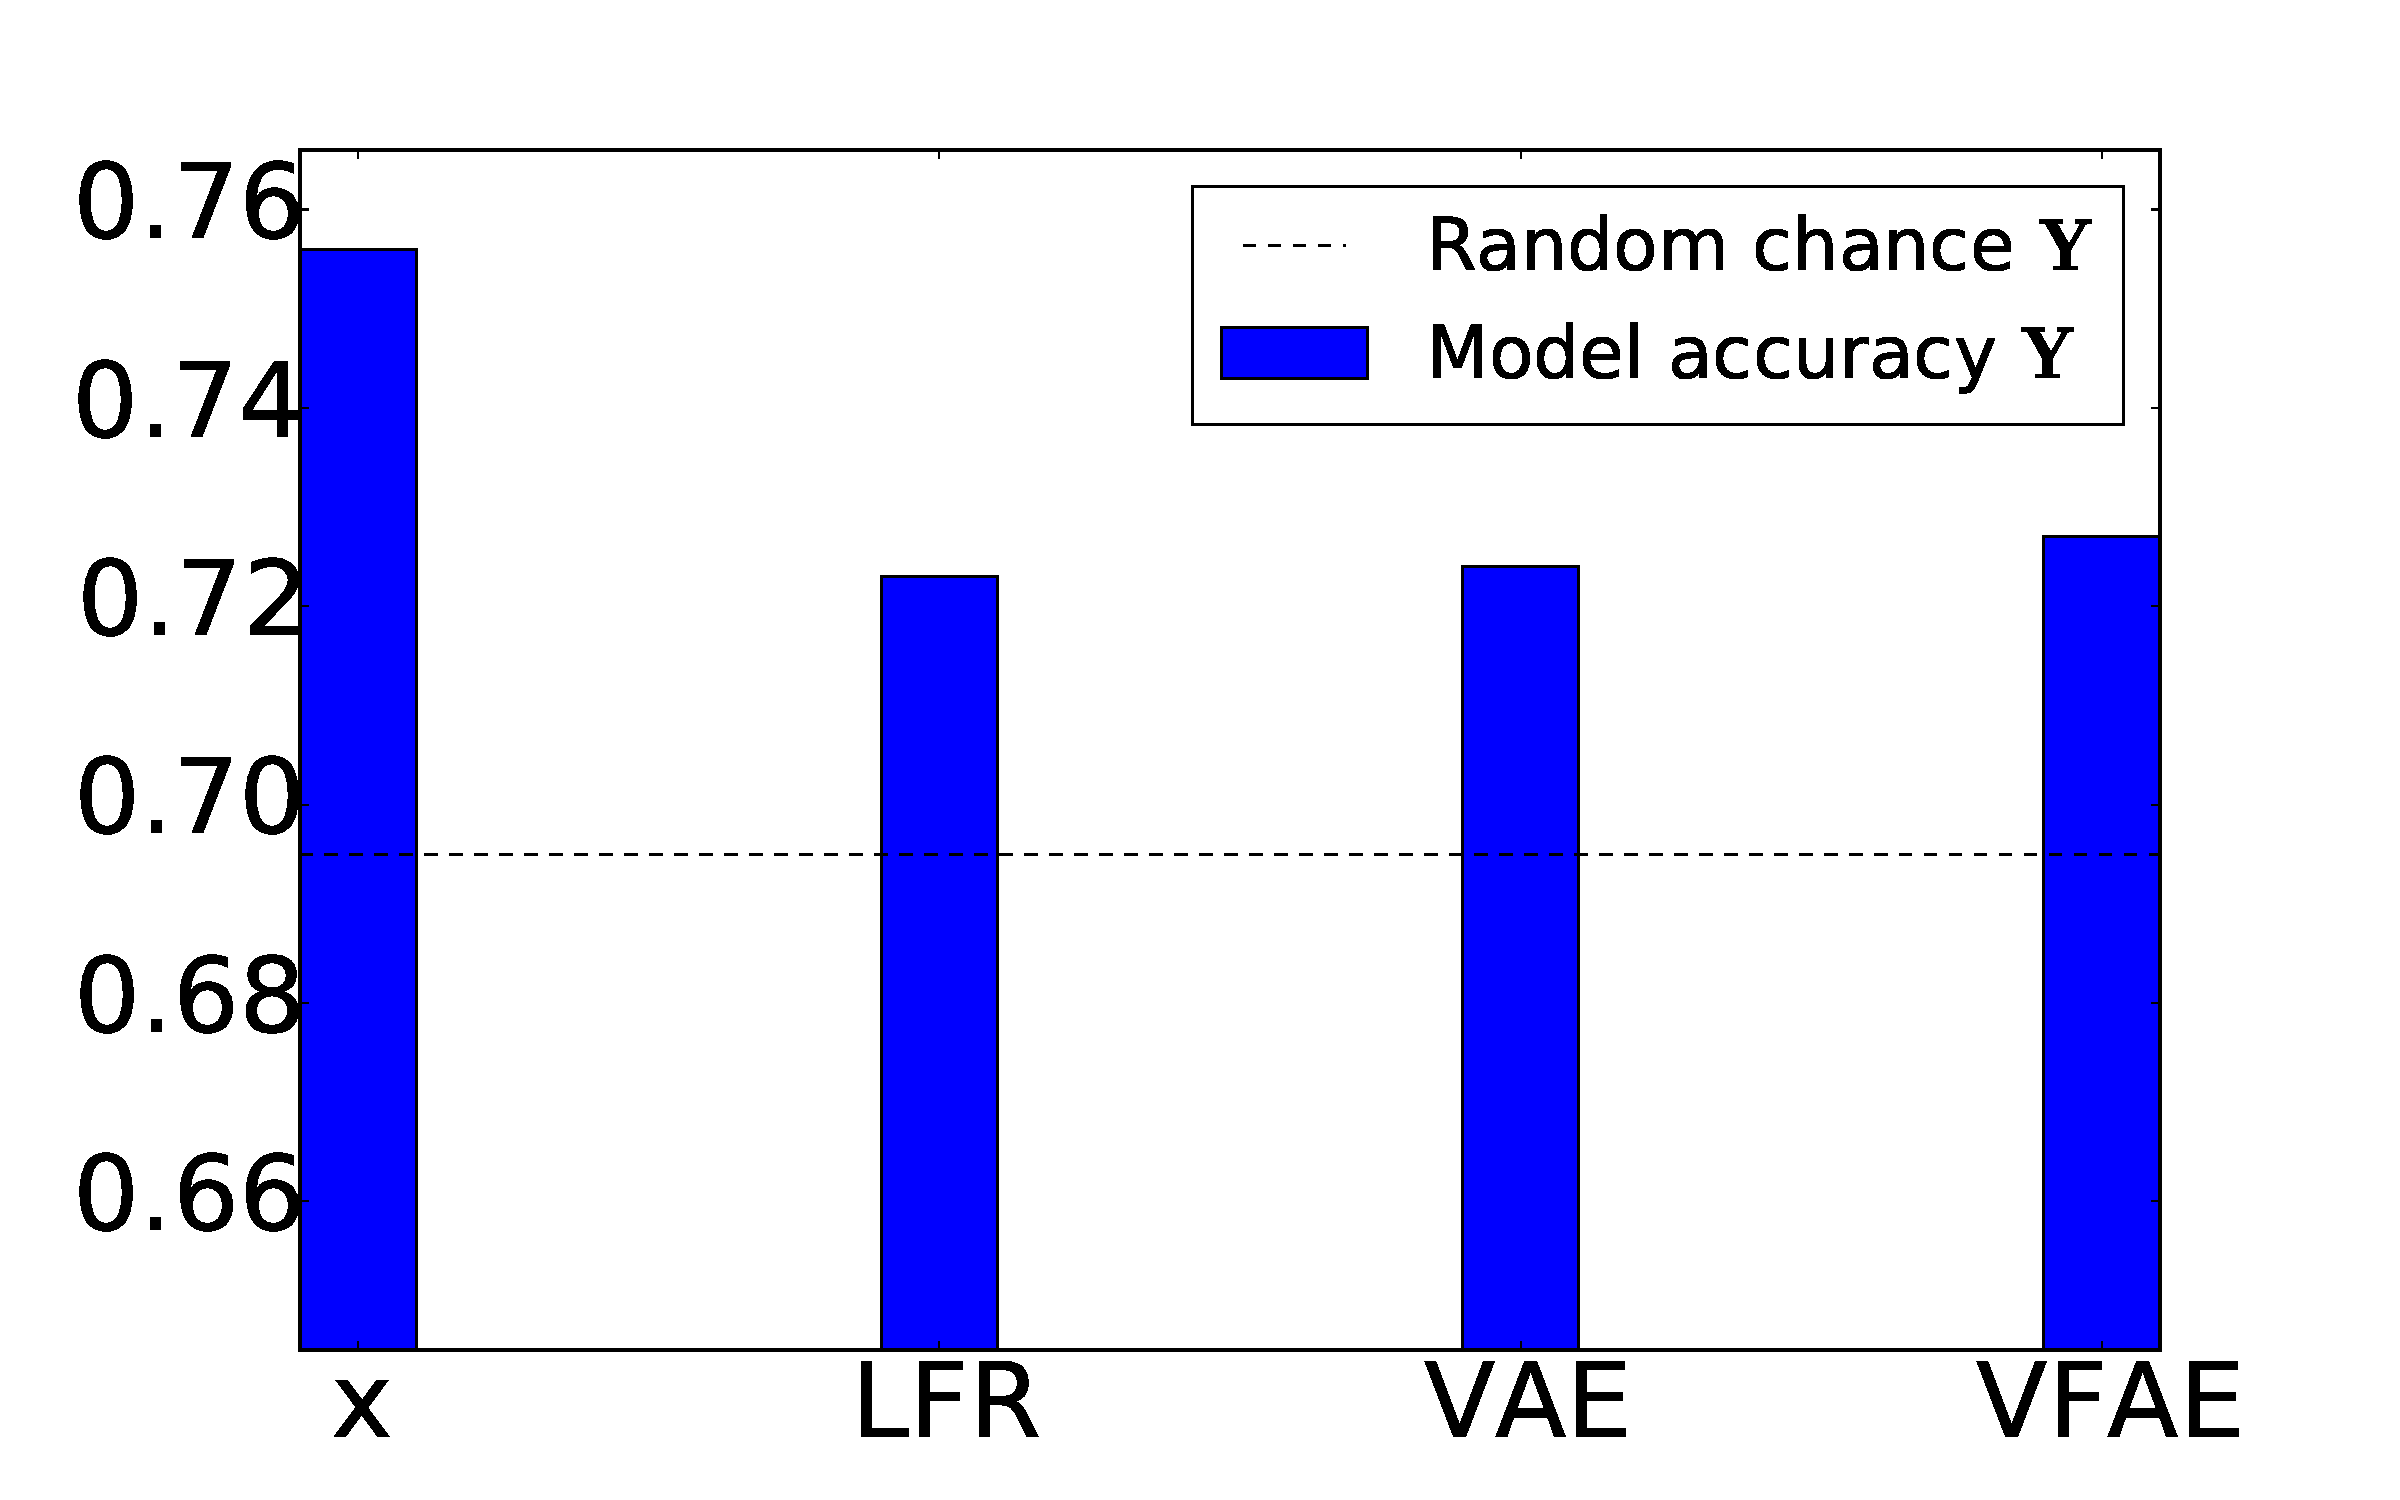
\includegraphics[width=1.1\linewidth]{german_y.pdf}
  \end{subfigure}
  \caption{German dataset}
  \end{subfigure}\\
  \begin{subfigure}{\linewidth}
  \begin{subfigure}{.329\textwidth}
      \centering
      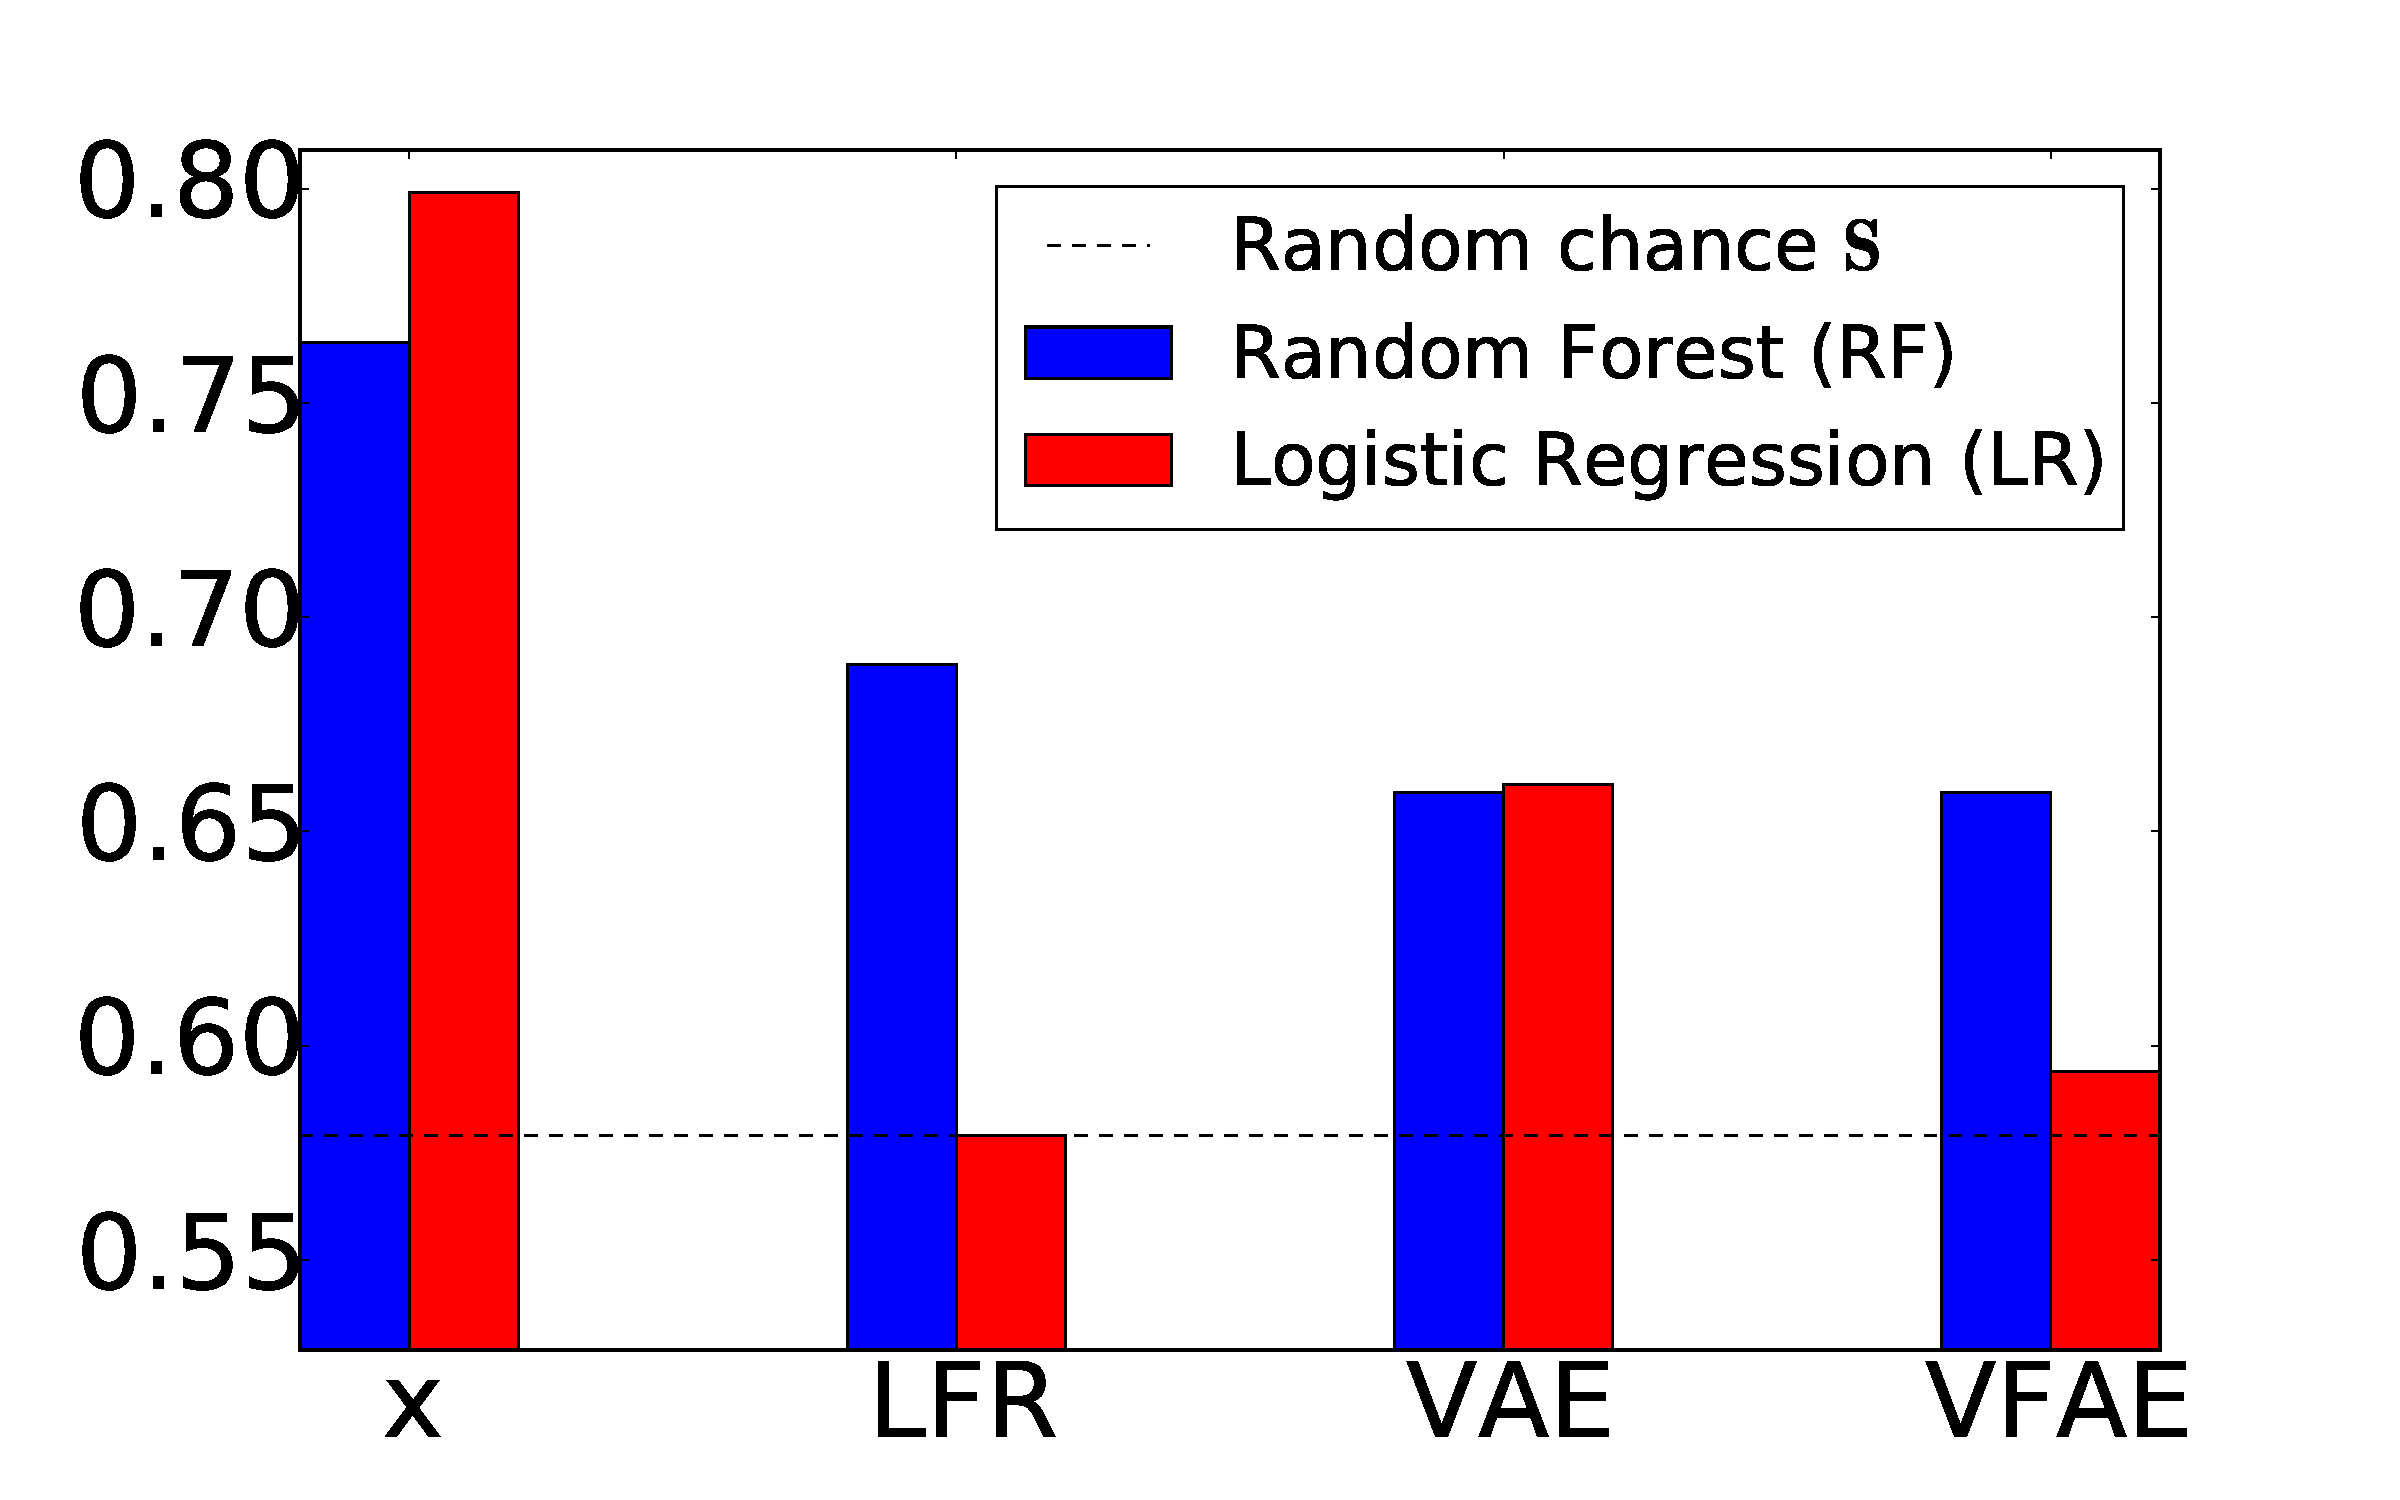
\includegraphics[width=1.1\linewidth]{health_s.pdf}
  \end{subfigure}%
  \begin{subfigure}{.329\textwidth}
      \centering
      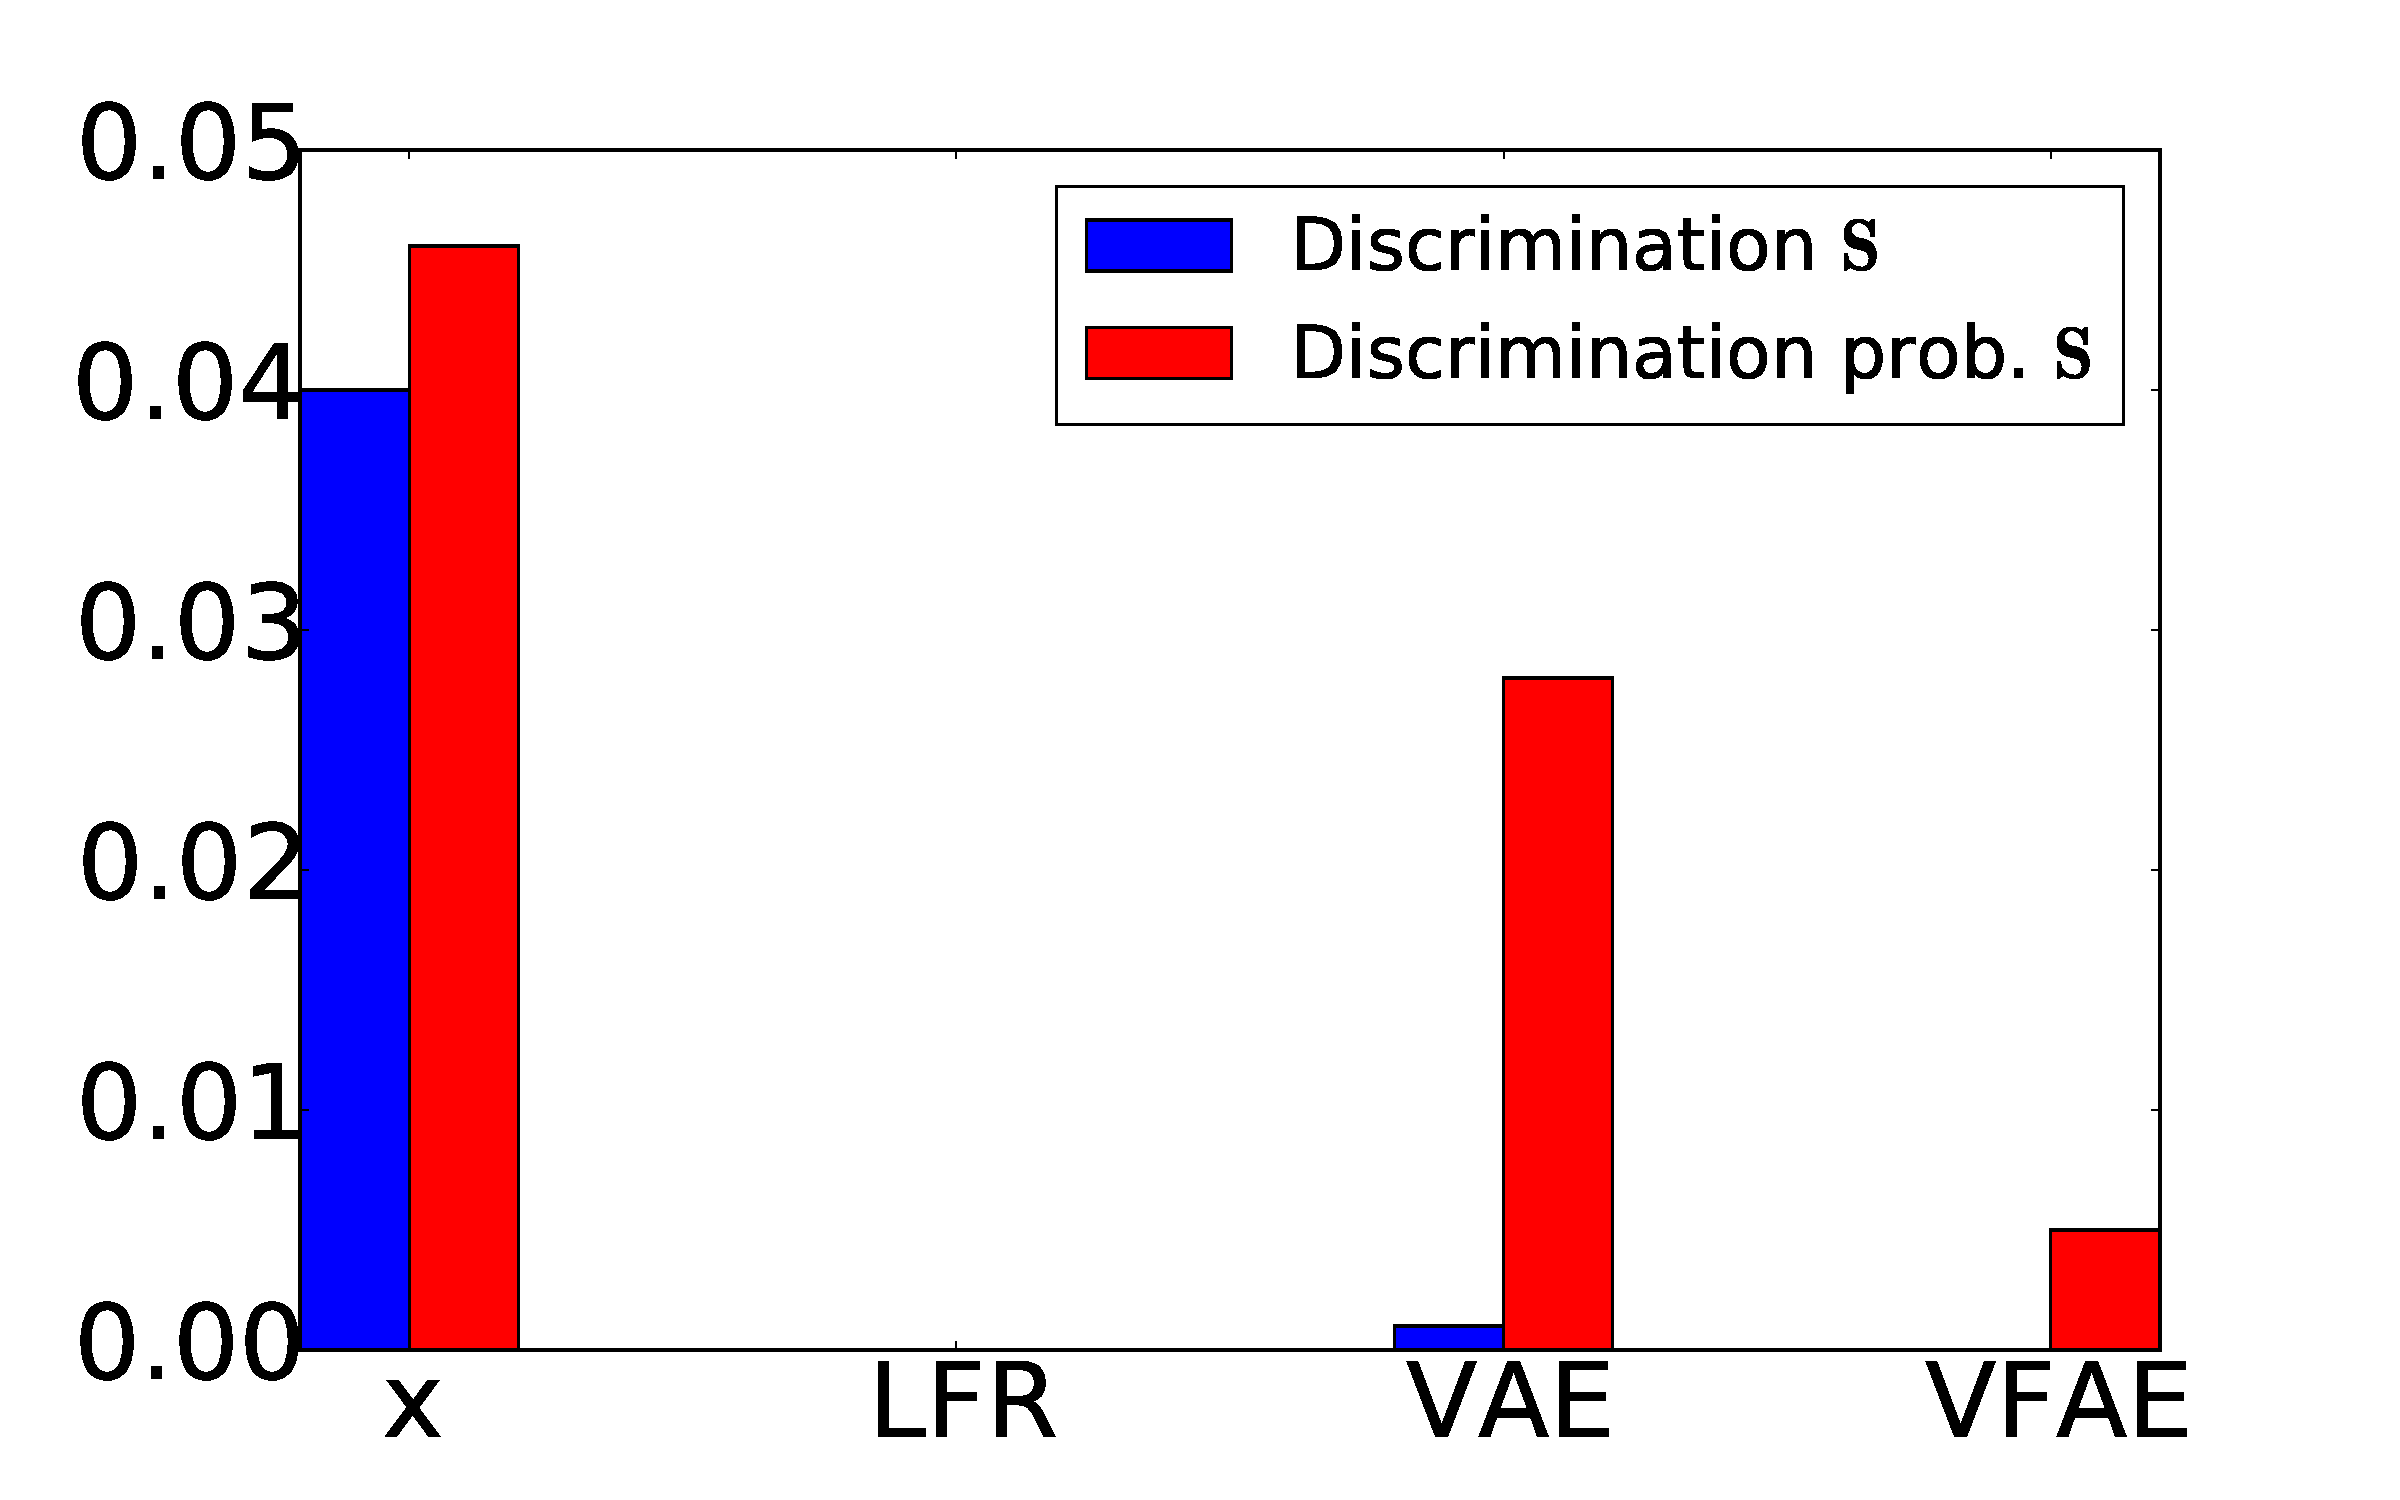
\includegraphics[width=1.1\linewidth]{health_discr.pdf}
  \end{subfigure}%
  \begin{subfigure}{.329\textwidth}
      \centering
      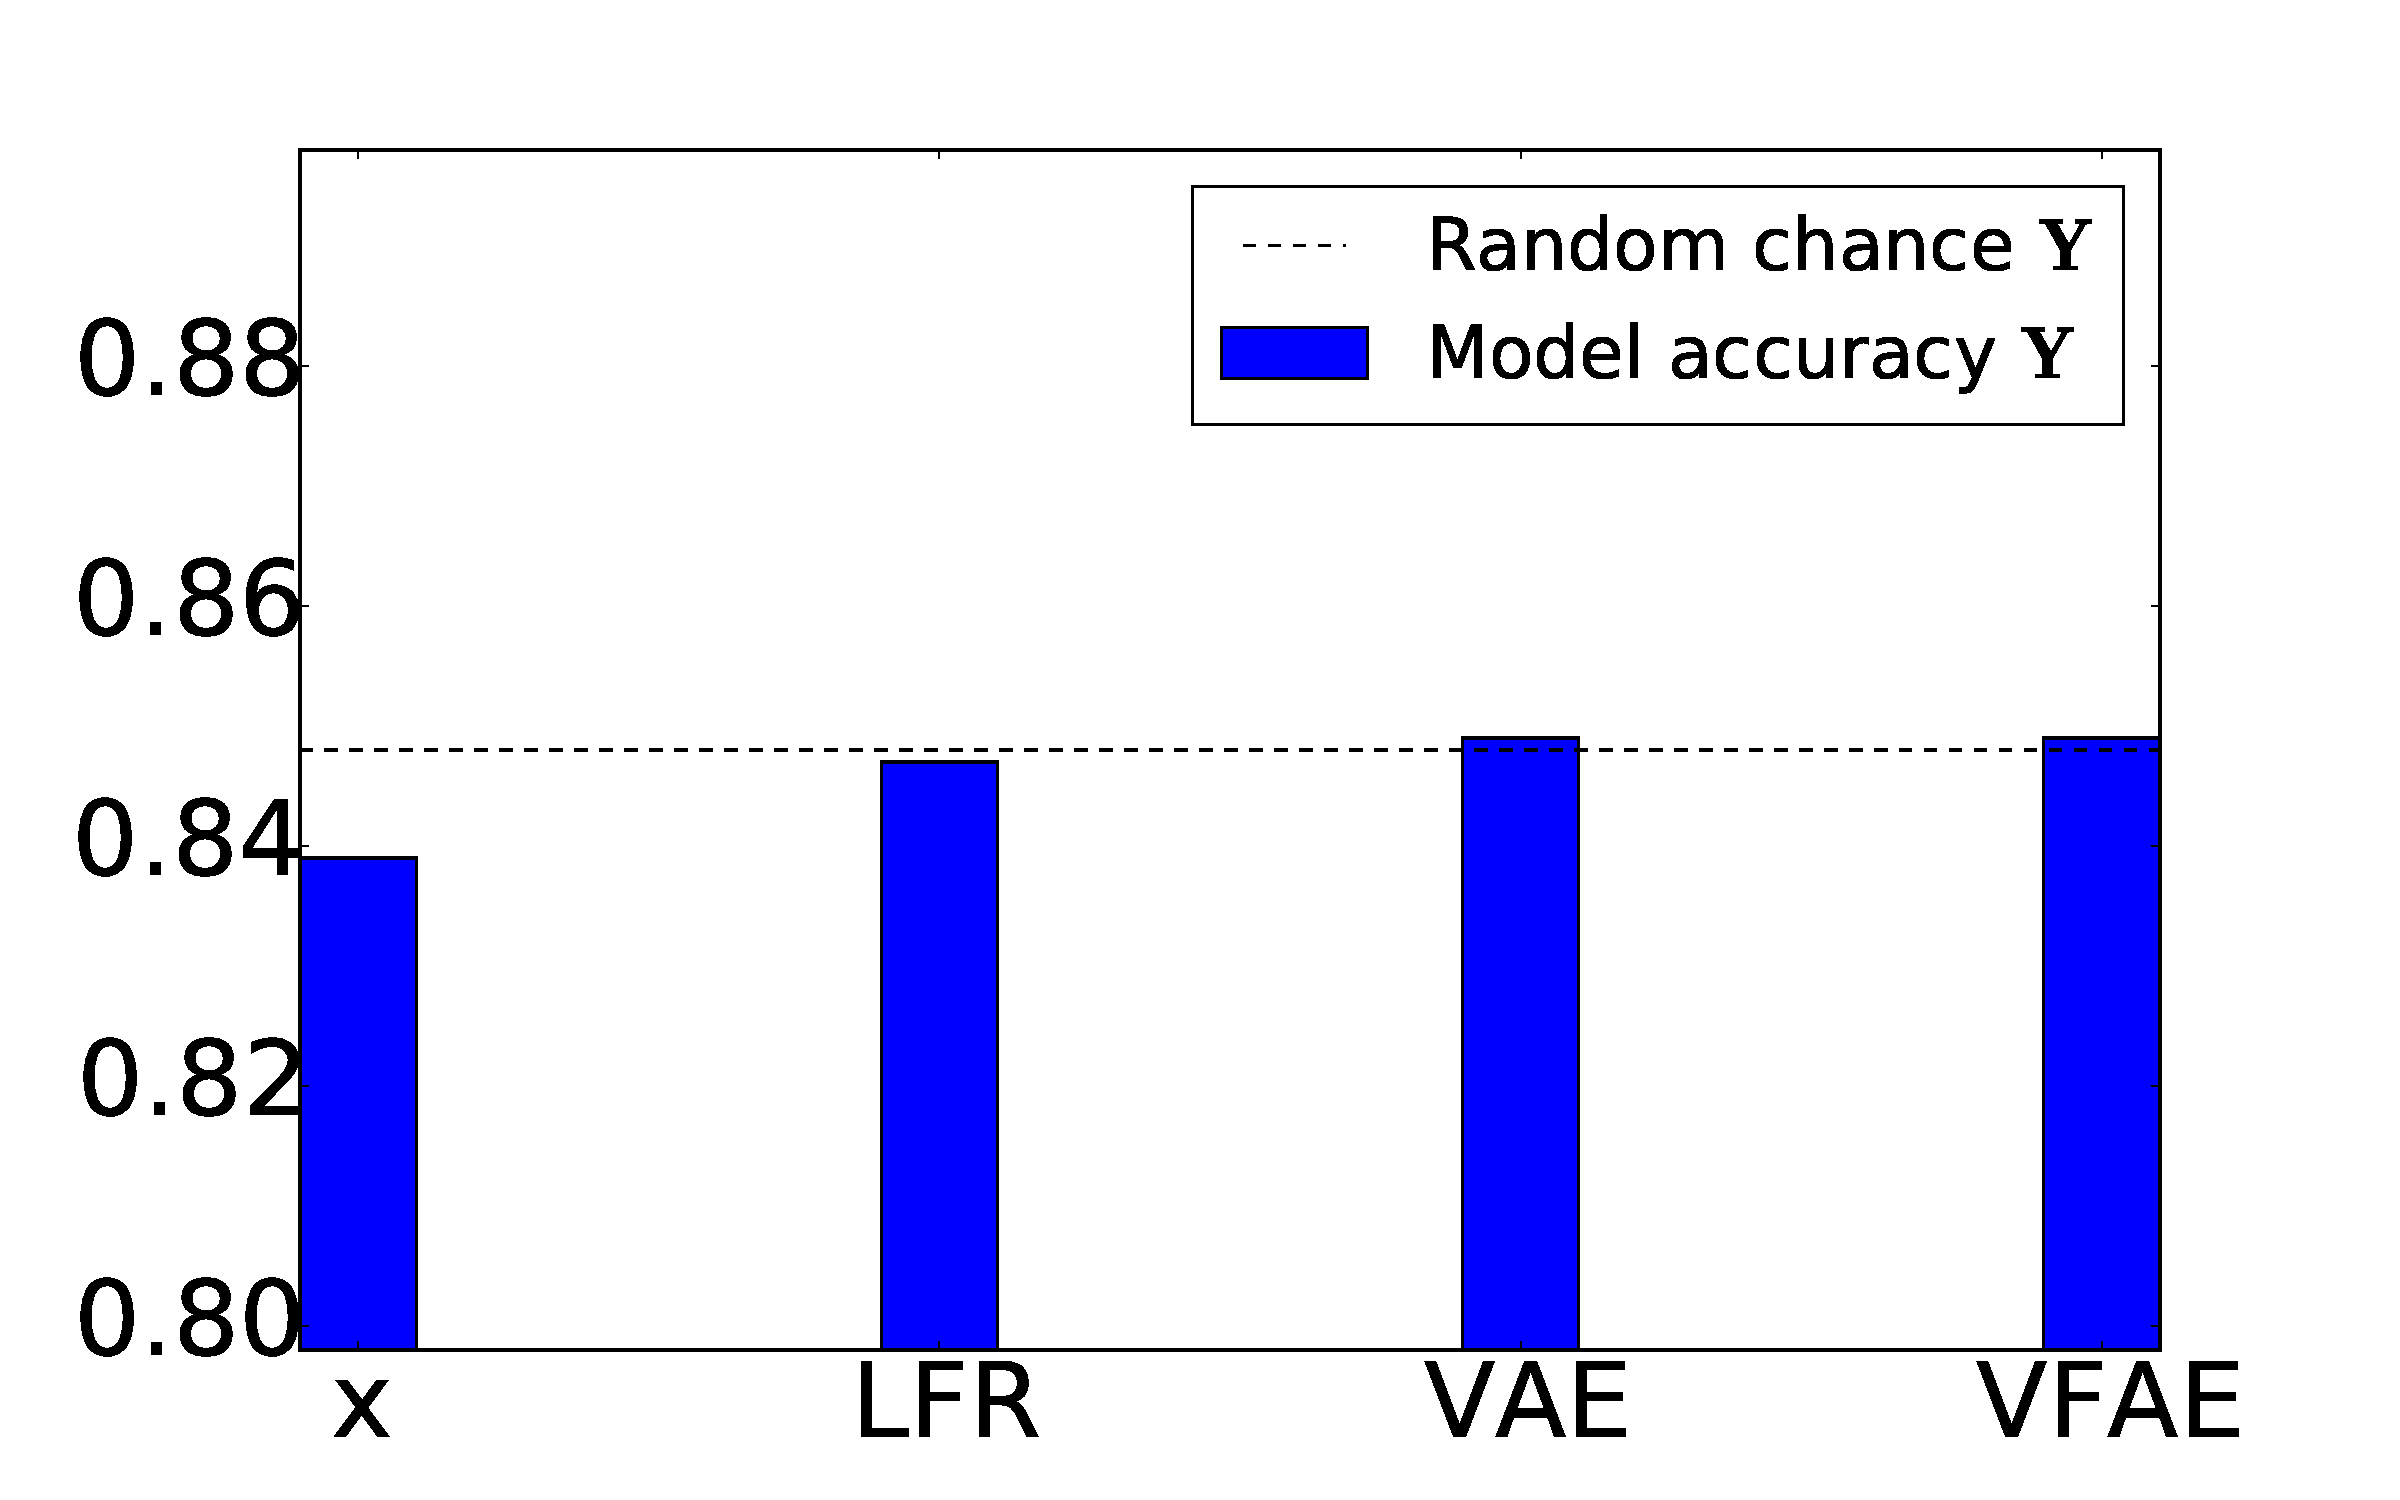
\includegraphics[width=1.1\linewidth]{health_y.pdf}
  \end{subfigure}
  \caption{Health dataset}
  \end{subfigure}%
  \caption{Fair classification results. Columns correspond to each evaluation scenario (in order): Random/RF/LR accuracy on $\*s$, Discrimination/Discrimination prob. against $\*s$ and Random/Model accuracy on $\*y$. Note that the objective of a ``fair'' encoding is to have low accuracy on S (where LR is a linear classifier and RF is nonlinear), low discrimination against S and high accuracy on Y.}
  \label{tab:fair_results}
\end{figure}

On the Adult dataset, the highest accuracy on the label $\*y$ and the lowest discrimination against $\*s$ is obtained by our LFR baseline. Despite the fact that LFR appears to give the best tradeoff between accuracy and discrimination, it appears to retain information about $\*s$ in its representation, which is discovered from the random forest classifier. In that sense, the VFAE method appears to do the best job in actually removing the sensitive information and maintaining most of the predictive information. Furthermore, the introduction of the MMD penalty in the VFAE model seems to provide a significant benefit with respect to our discrimination metrics, as both were reduced considerably compared to the regular VAE. 

On the German dataset, all methods appear to be invariant with respect to the sensitive information $\*s$. However this is not the case for the discrimination metric, since LFR does appear to retain information compared to the VAE and VFAE. The MMD penalty in VFAE did seem improve the discrimination scores over the original VAE, while the accuracy on the labels $\*y$ remained similar. 

As for the Health dataset; this dataset is extremely imbalanced, with only 15\% of the patients being admitted to a hospital. Therefore, each of the classifiers seems to predict the majority class as the label $\*y$ for every point. For the invariance against $\*s$ however, the results were more interesting. On the one hand, the VAE model on this dataset did maintain some sensitive information, which could be identified both linearly and non-linearly. On the other hand, VFAE and the LFR methods were able to retain less information in their latent representation, since only Random Forest was able to achieve higher than random chance accuracy. This further justifies our choice for including the MMD penalty in the lower bound of the VAE. .

In order to further assess the nature of our new representations, we visualized two dimensional Barnes-Hut SNE~\citep{2013arXiv1301.3342V} embeddings of the $\*z_1$ representations, obtained from the model trained on the Adult dataset, in Figure~\ref{fig:tsne_adult_all}. As we can see, the nuisance/sensitive variables $\*s$ can be identified both on the original representation $\*x$ and on a latent representation $\*z_1$ that does not have the MMD penalty and the independence properties between $\*z_1$ and $\*s$ in the prior. By introducing these independence properties as well as the MMD penalty the nuisance variable groups become practically indistinguishable.

\begin{figure}[h]
  \centering
  \begin{subfigure}{.25\textwidth}
        \centering
        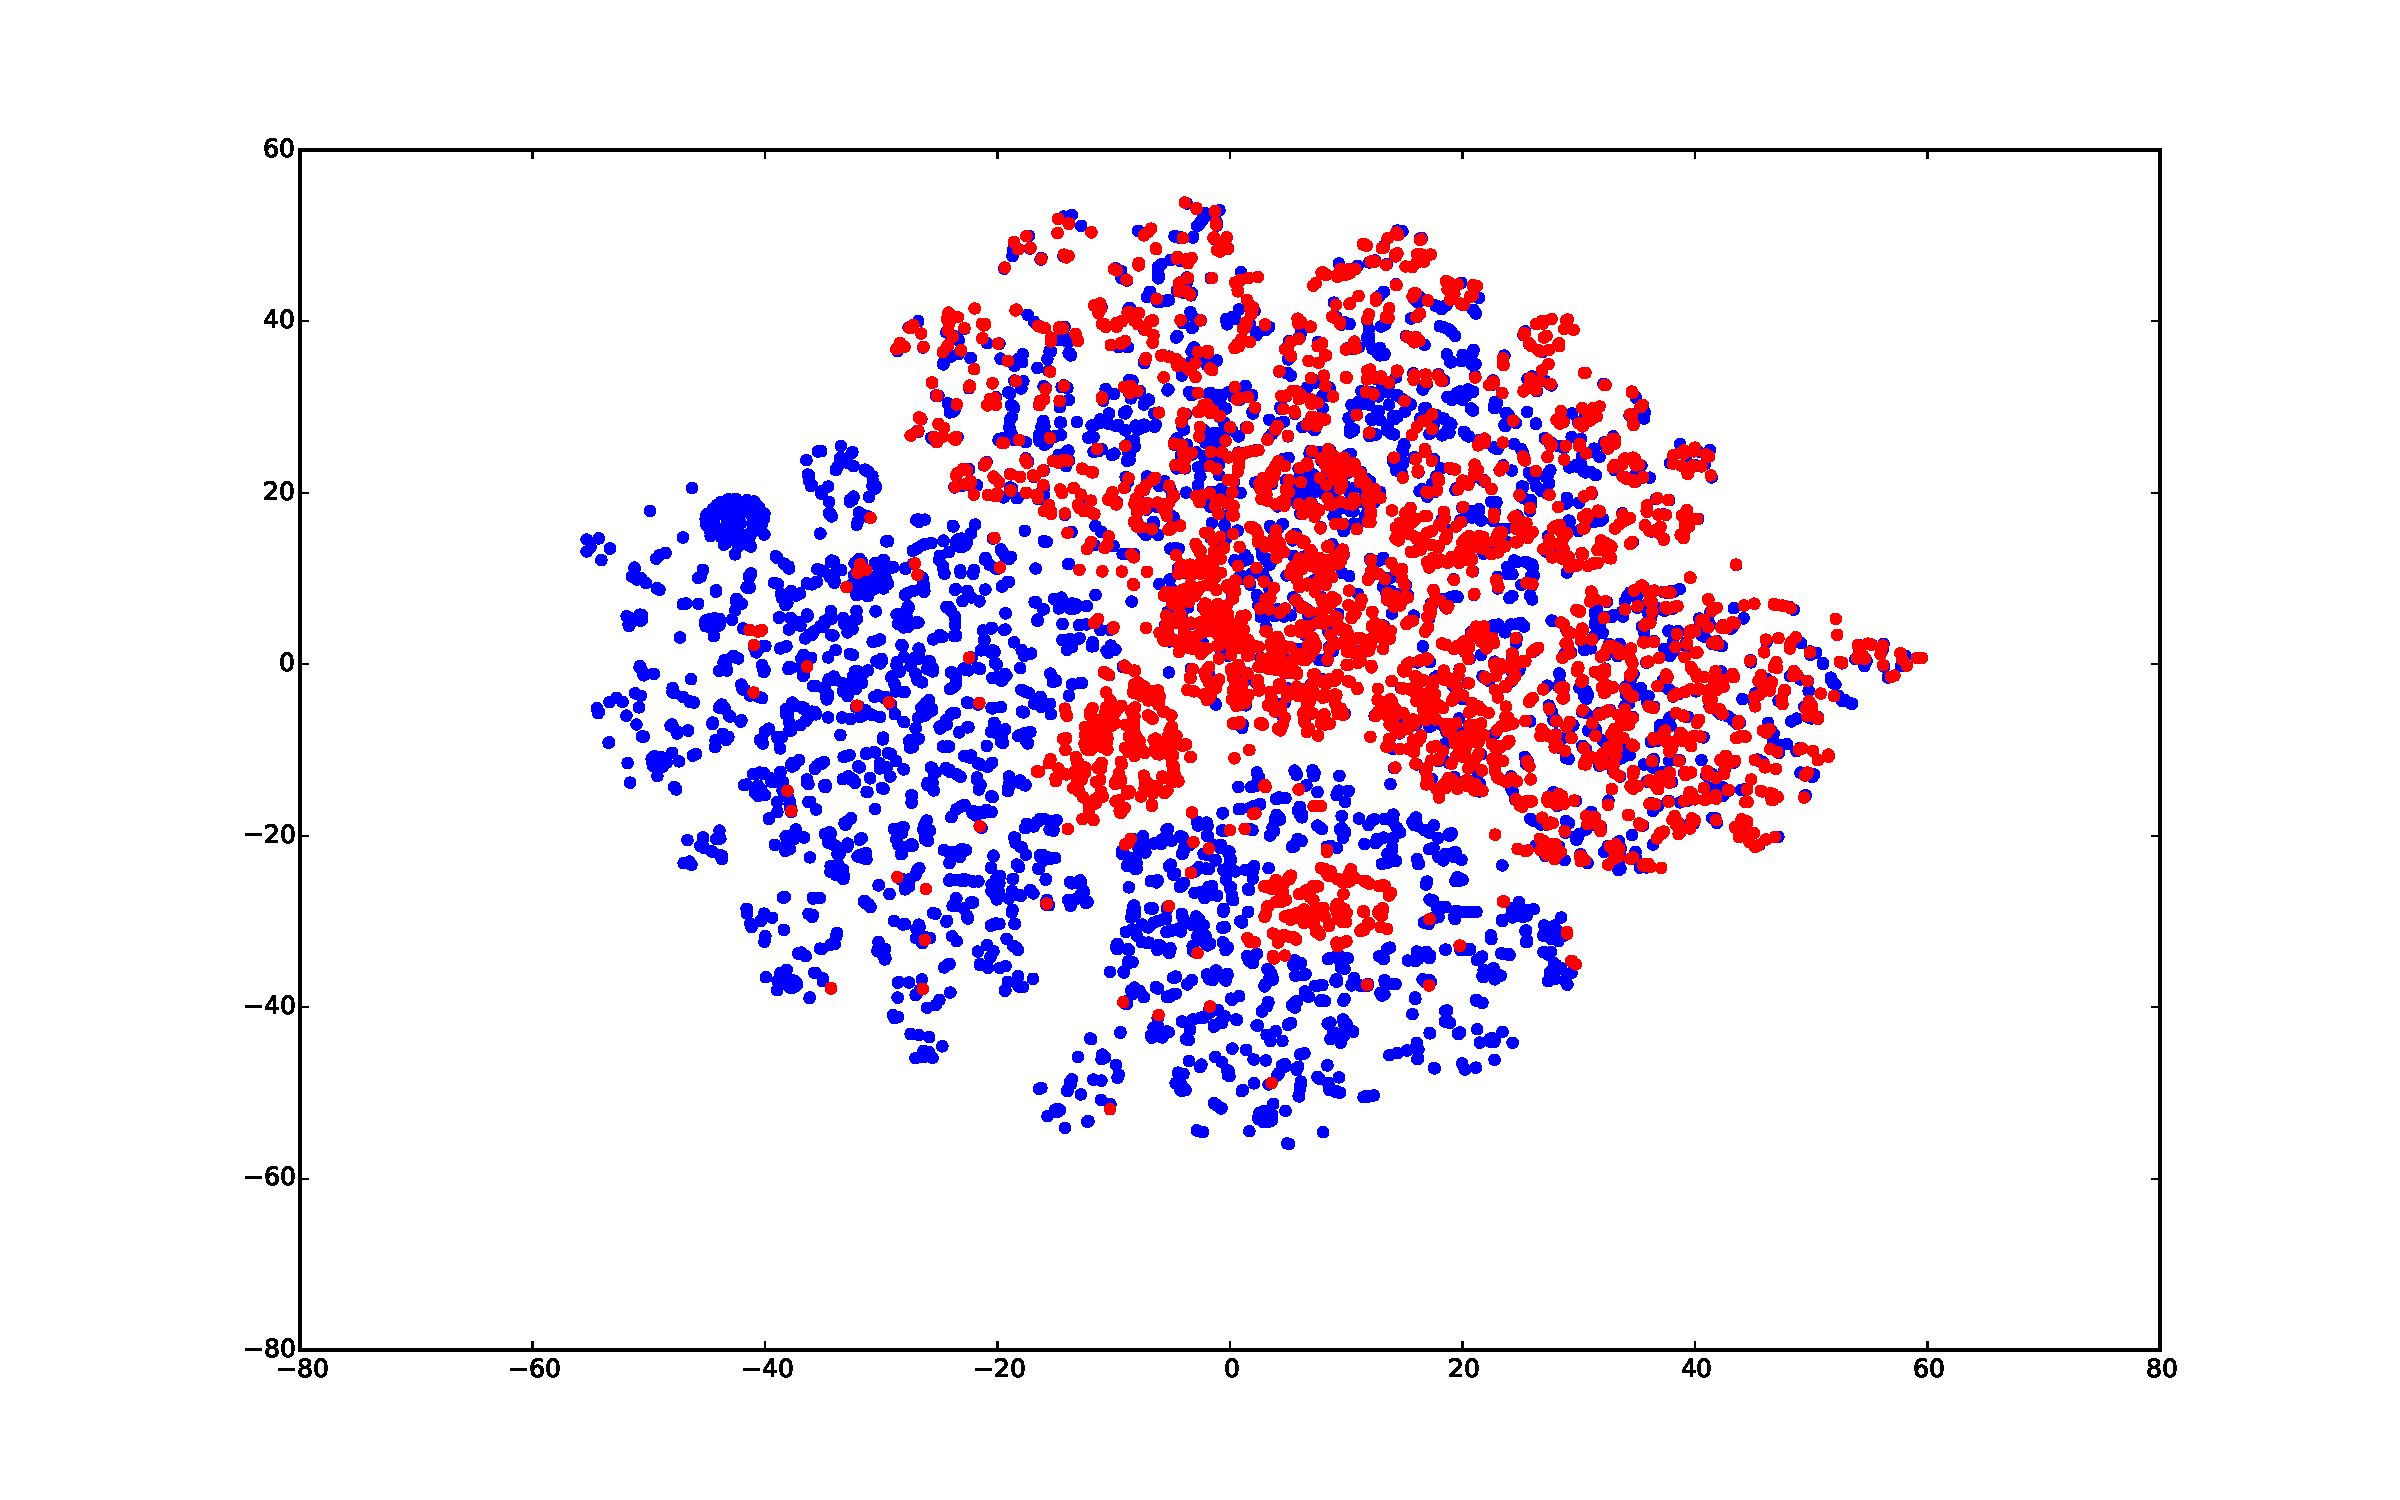
\includegraphics[width=1.\textwidth]{tsne_adult_x.pdf}
        \caption{}
        \label{fig:tsne_adult_x}
    \end{subfigure}%
    \begin{subfigure}{.25\textwidth}
        \centering
        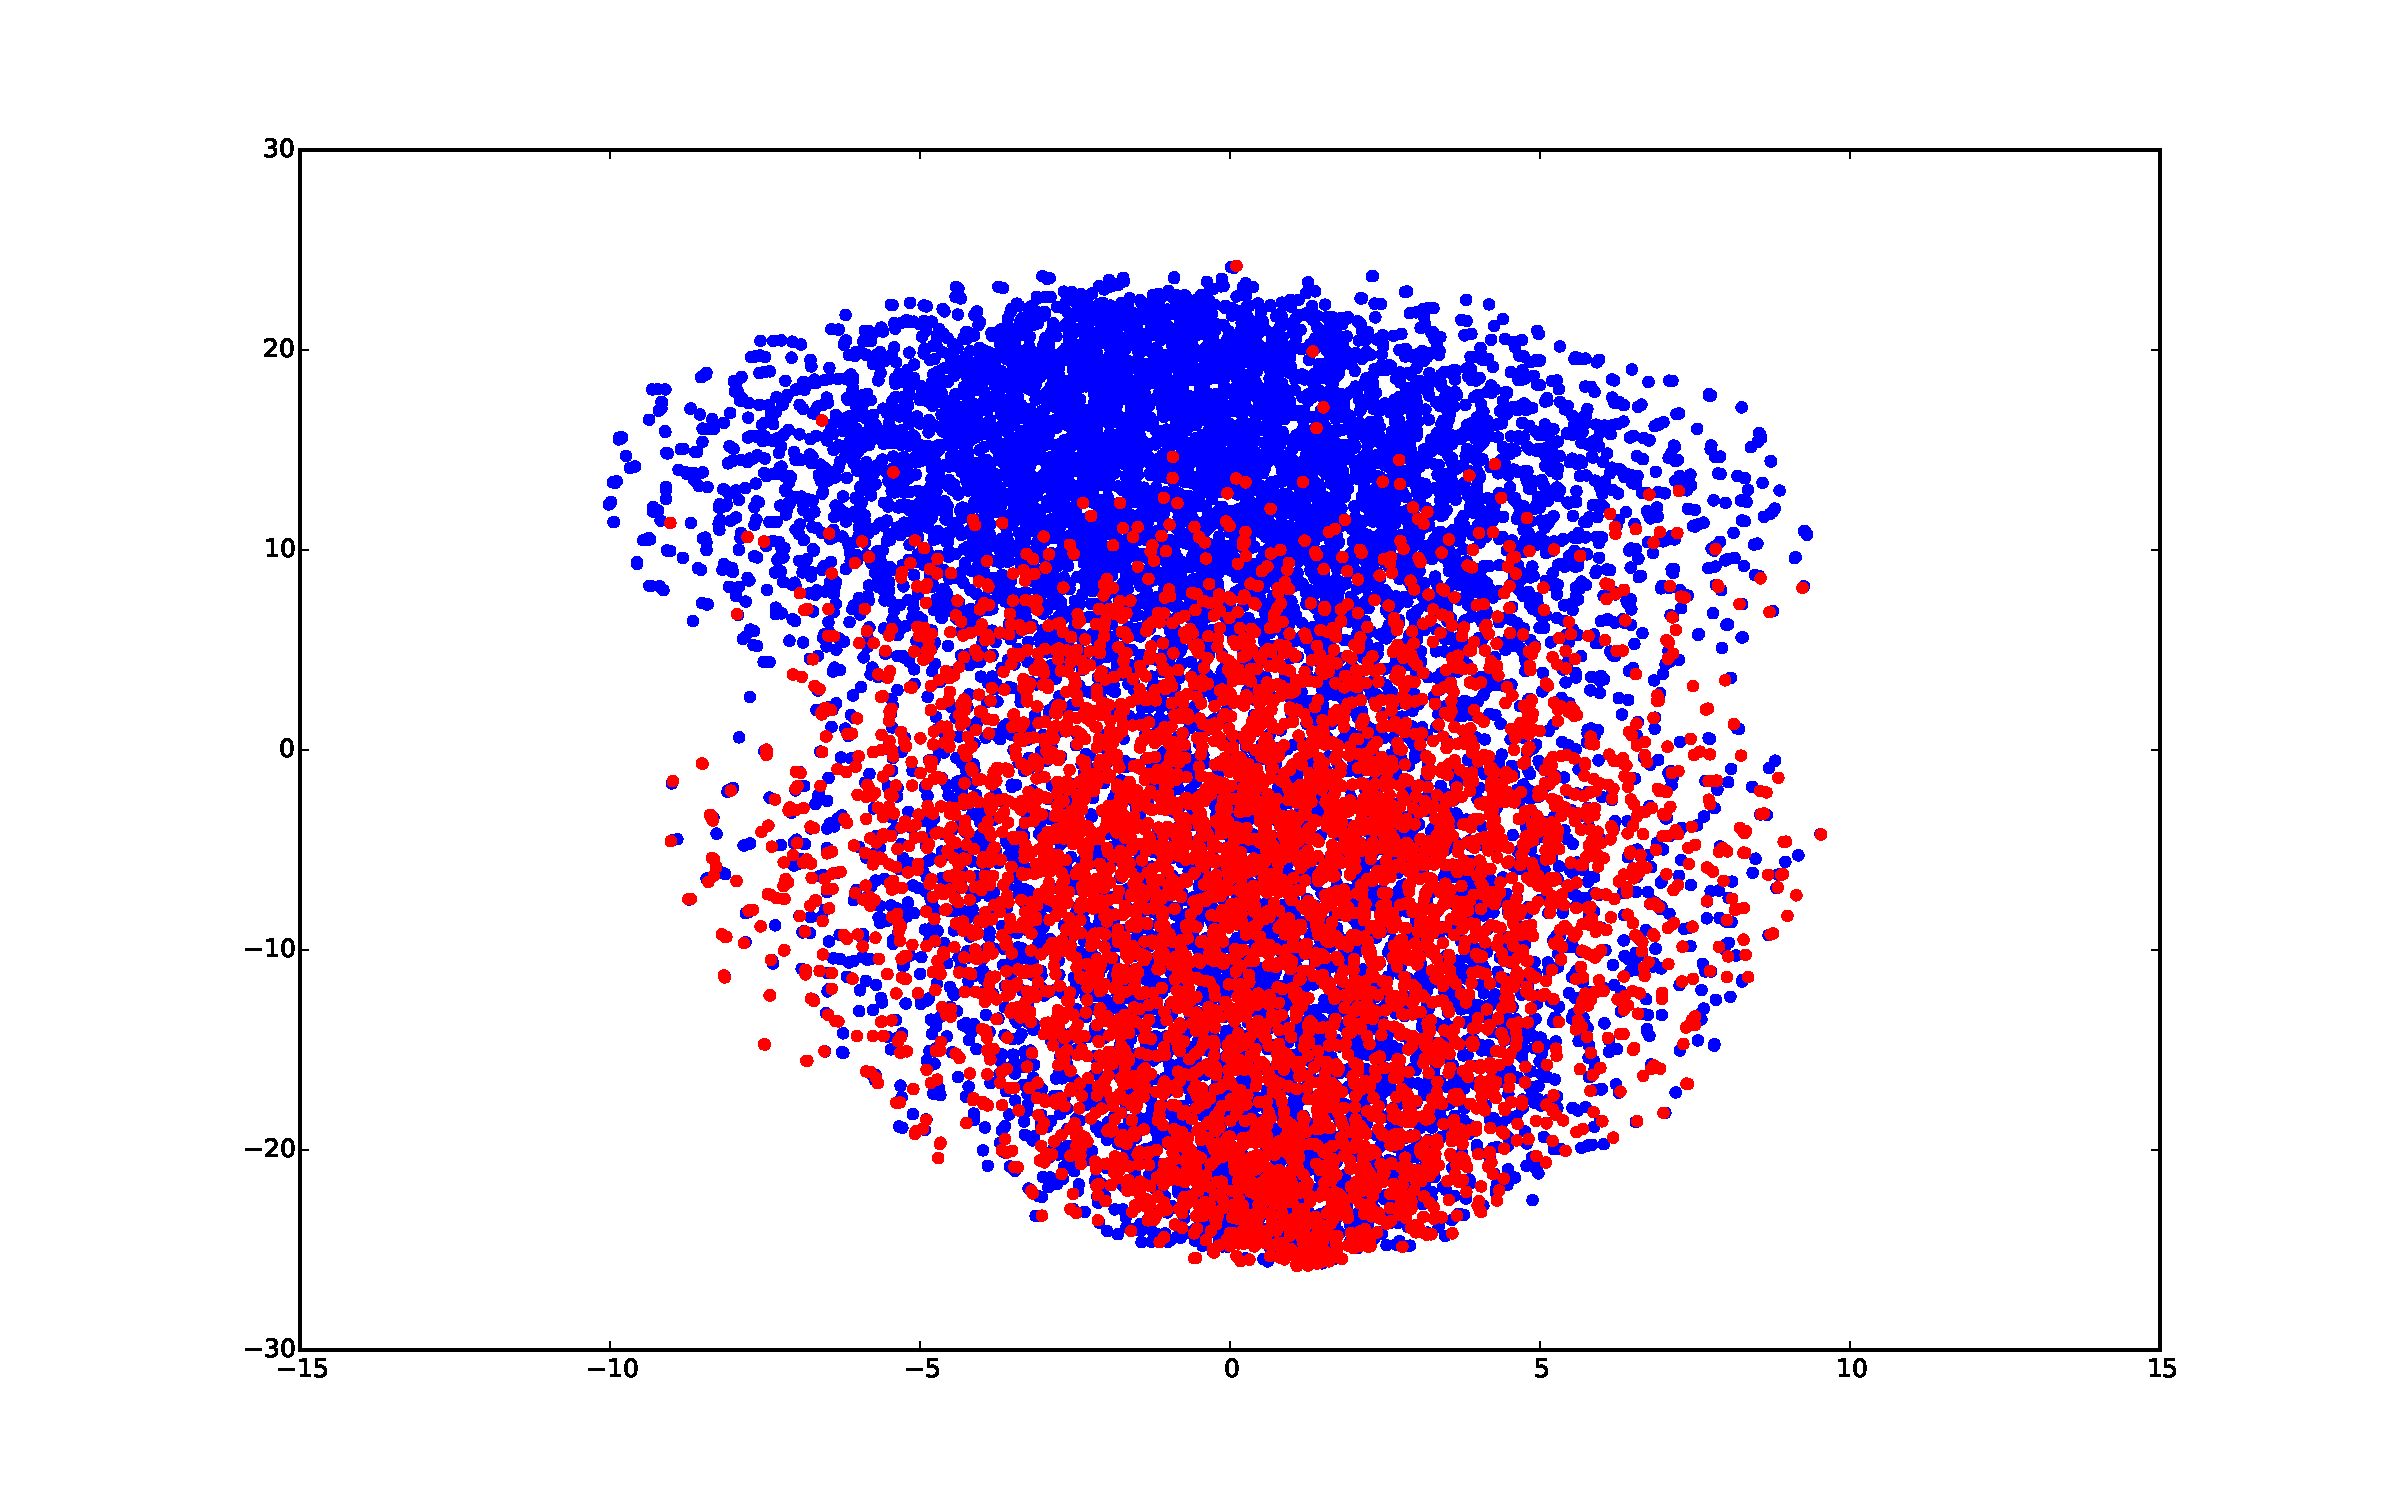
\includegraphics[width=1.\textwidth]{tsne_adult.pdf}
        \caption{}
        \label{fig:tsne_adult}
    \end{subfigure}%
    \begin{subfigure}{.25\textwidth}
        \centering
        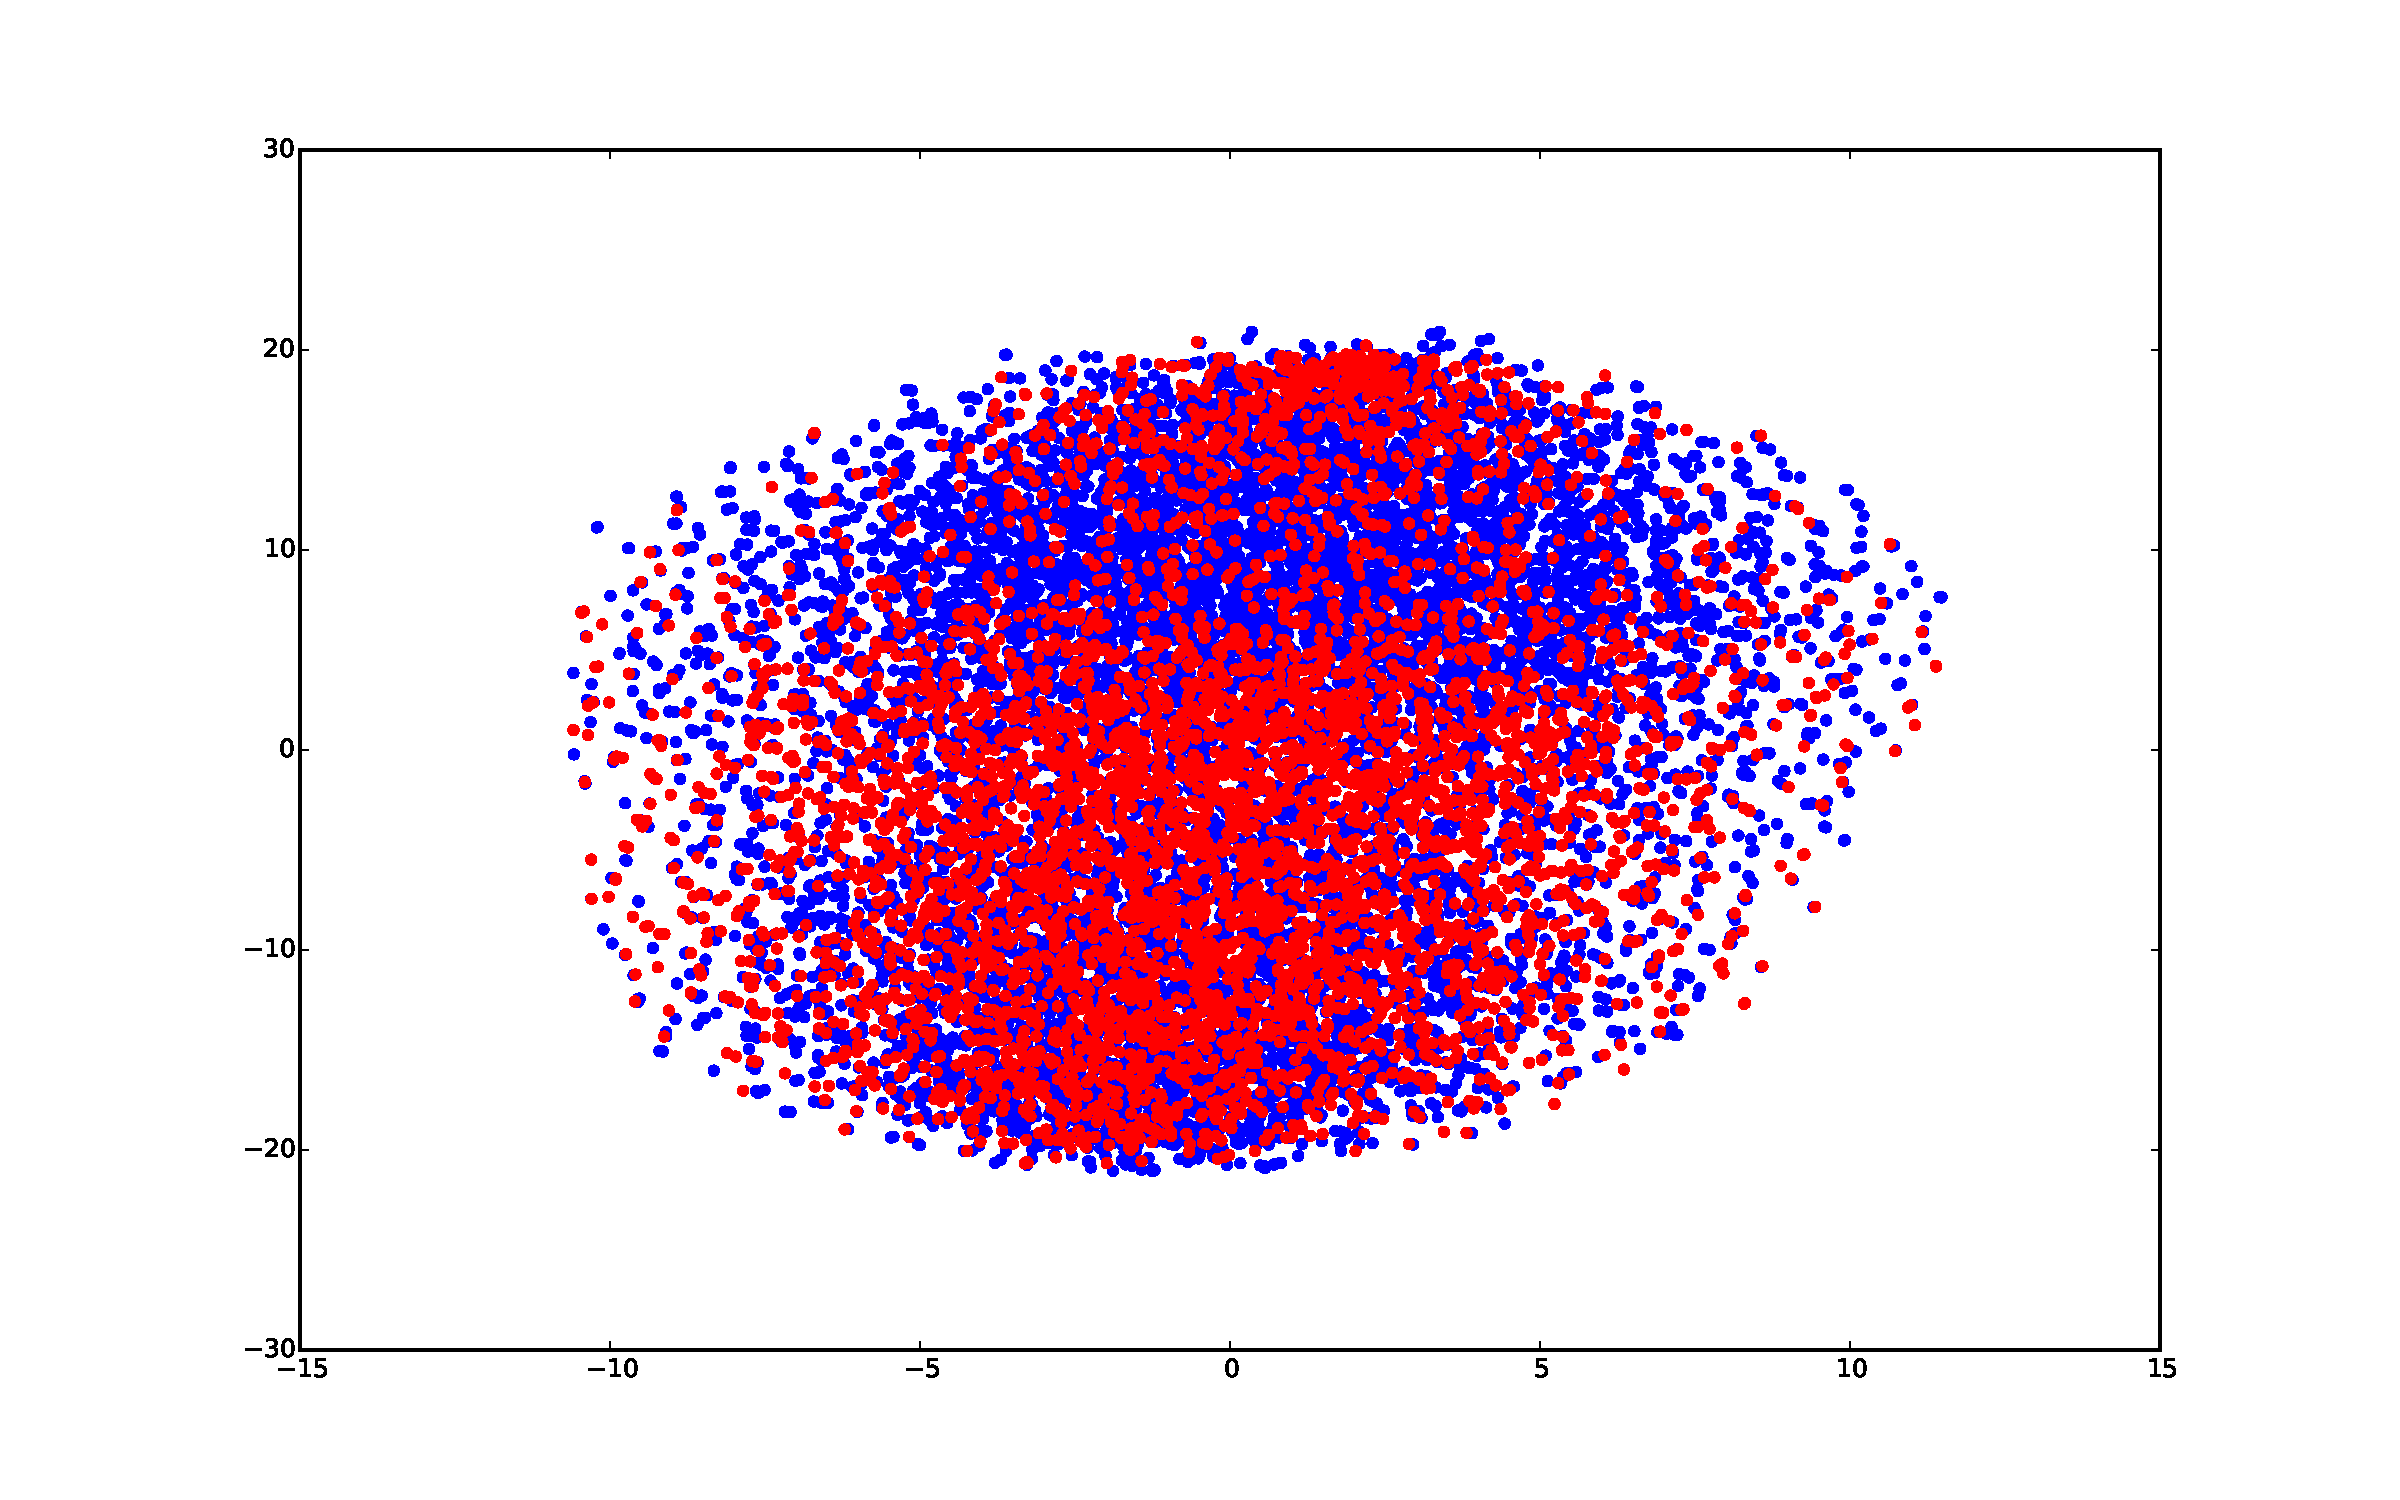
\includegraphics[width=1.\textwidth]{tsne_adult_s.pdf}
        \caption{}
        \label{fig:tsne_adult_s}
    \end{subfigure}%
    \begin{subfigure}{.25\textwidth}
        \centering
        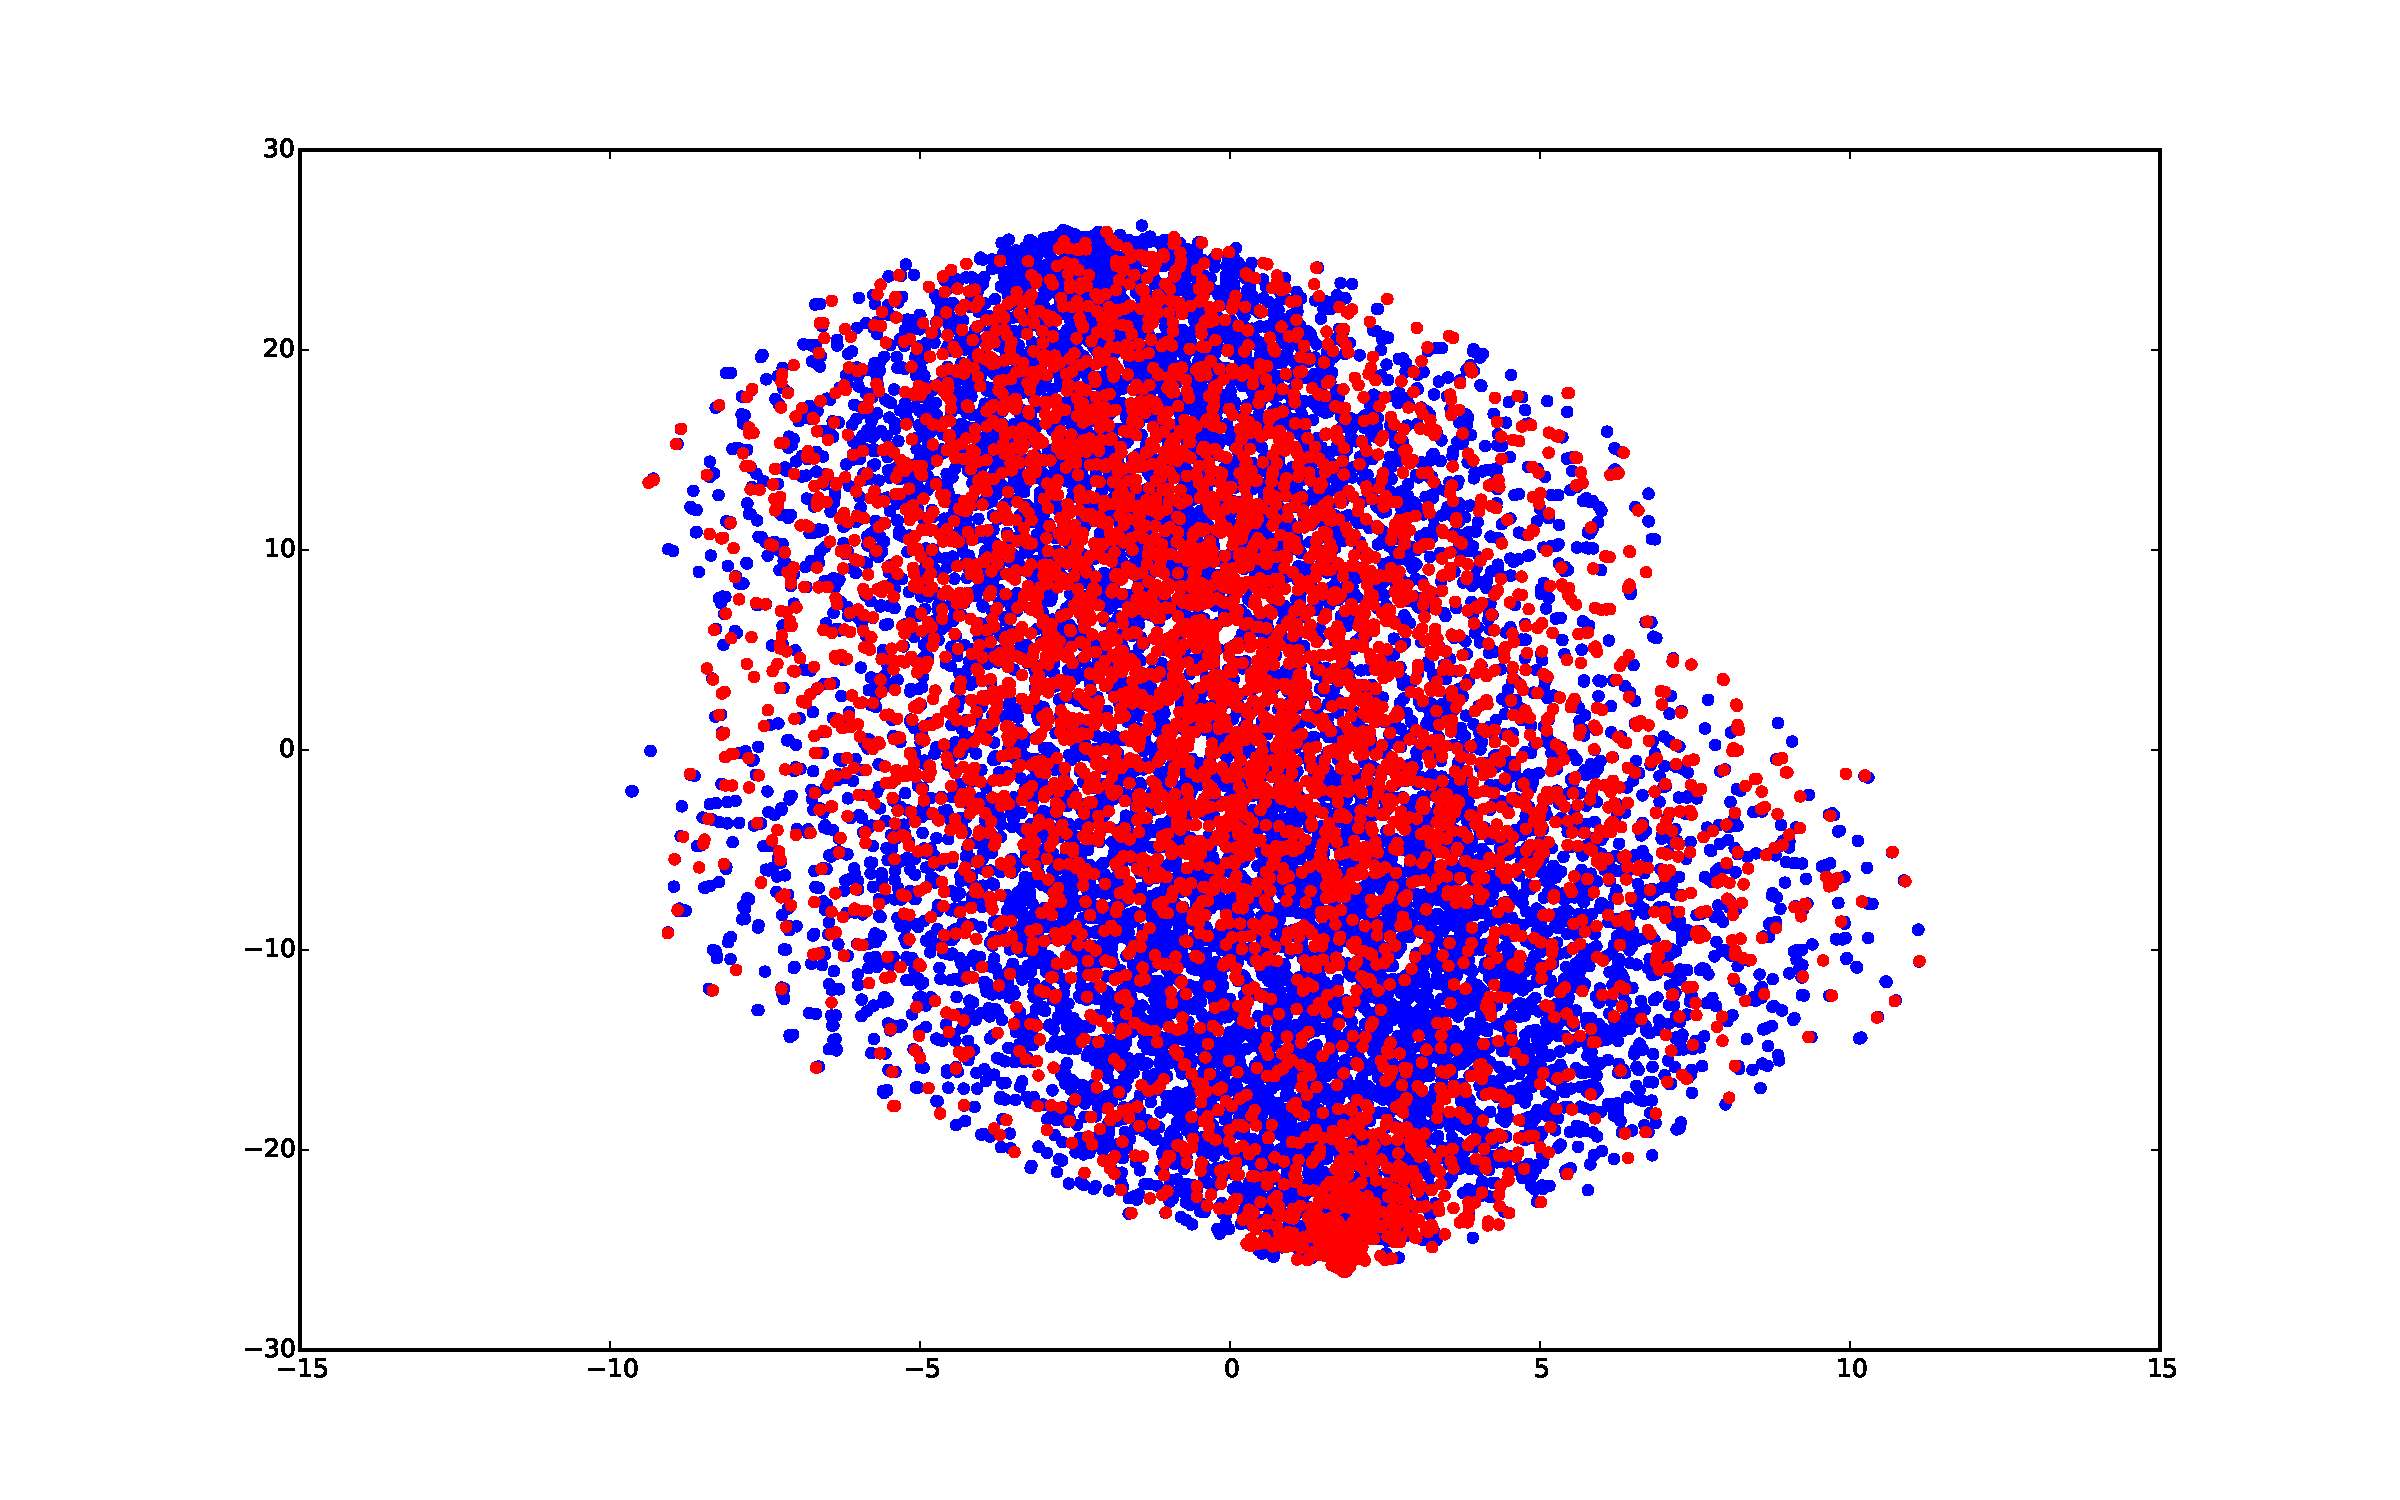
\includegraphics[width=1.\textwidth]{tsne_adult_mmd_s.pdf}
        \caption{}
        \label{fig:tsne_adult_mmd_s}
    \end{subfigure}%
    \caption{t-SNE~\citep{2013arXiv1301.3342V} visualizations from the Adult dataset on: (a): original $\*x$ , (b):  latent $\*z_1$  without $\*s$ and MMD, (c): latent $\*z_1$ with $\*s$ and without MMD, (d):  latent $\*z_1$ with $\*s$ and MMD. Blue colour corresponds to males whereas red colour corresponds to females.}
    \label{fig:tsne_adult_all}
\end{figure}

\subsubsection{Domain adaptation}
As for the domain adaptation scenario and the Amazon reviews dataset, the results of our VFAE model can be seen in Table~\ref{tab:amazon_results}. Our model was successful in factoring out the domain information, since the accuracy, measured both linearly (LR) and non-linearly (RF), was towards random chance (which for this dataset is 0.5).  We should also mention that, on this dataset at least, completely removing information about the domain does not guarantee a better performance on $\*y$. The same effect was also observed by~\cite{2015arXiv150507818G} and~\cite{chen2012marginalized}. As far as the accuracy on $\*y$ is concerned, we compared against a recent neural network based state of the art method for domain adaptation, Domain Adversarial Neural Network (DANN)~\citep{2015arXiv150507818G}. As we can observe in table~\ref{tab:amazon_results}, our accuracy on the labels $\*y$ is higher on 9 out of the 12 domain adaptation tasks whereas on the remaining 3 it is quite similar to the DANN architecture. 

\begin{table}[ht]
	\caption {Results on the Amazon reviews dataset. The DANN column is taken directly from~\cite{2015arXiv150507818G} (the column that uses the original representation as input).}
	\centering
	\label{tab:amazon_results}
	\begin{center}
		\begin{tabular}{l|l|l|l|l}
			\hline
			\multirow{2}{*}{Source - Target}  & \multicolumn{2}{c|}{S}  & \multicolumn{2}{c}{Y}  \\\cline{2-5}
			& RF & LR & VFAE & DANN \\\hline
			books - dvd & 0.535 & 0.564 & \textbf{0.799} & 0.784 \\ 
			books - electronics & 0.541 & 0.562 & \textbf{0.792} & 0.733 \\
			books - kitchen & 0.537 & 0.583 &  \textbf{0.816} & 0.779 \\
			dvd - books & 0.537 & 0.563 & \textbf{0.755} & 0.723 \\
			dvd - electronics & 0.538 & 0.566 & \textbf{0.786} & 0.754\\
			dvd - kitchen & 0.543 & 0.589 &  \textbf{0.822} & 0.783\\
			electronics - books & 0.562 & 0.590  & \textbf{0.727} & 0.713\\
			electronics - dvd & 0.556 & 0.586 & \textbf{0.765} & 0.738\\
			electronics - kitchen & 0.536 & 0.570 & 0.850 & \textbf{0.854}\\ 
			kitchen - books & 0.560 & 0.593 & \textbf{0.720} & 0.709  \\
			kitchen - dvd & 0.561 & 0.599 & 0.733 & \textbf{0.740} \\
			kitchen - electronics & 0.533 & 0.565  & 0.838 & \textbf{0.843} \\
			\hline
		\end{tabular}
		\end{center}
\end{table}

\subsection{Learning Invariant Representations}
Regarding the more general task of learning invariant representations; our results on the Extended Yale B dataset also demonstrate our model's ability to learn such representations. As expected, on the original representation $\*x$ the lighting conditions, $\*s$, are well identifiable with almost perfect accuracy from both RF and LR. This can also be seen in the two dimensional embeddings of the original space $\*x$ in Figure~\ref{fig:yaleb_x}: the images are mostly clustered according to the lighting conditions. As soon as we utilize our VFAE model we simultaneously decrease the accuracy on $\*s$, from 96\% to about 50\%, and increase our accuracy on $\*y$, from 78\% to about 85\%. This effect can also be seen in Figure~\ref{fig:yaleb_z}: the images are now mostly clustered according to the person ID (the label $\*y$). It is clear that in this scenario the information about  $\*s$ is purely ``nuisance'' with respect to the labels $\*y$. Therefore, by using our VFAE model we are able to obtain improved generalization and classification performance by effectively removing $\*s$ from our representations.
   
\begin{table}[ht]
	\caption {Results on the Extended Yale B dataset. We also included the best result from~\cite{li2014learning} under the NN + MMD row.}
	\centering
	\label{tab:yaleb_results}
	\begin{center}
		\begin{tabular}{l|l|l|l}
			\hline
			\multirow{2}{*}{Method}  & \multicolumn{2}{c|}{S}  &  \multirow{2}{*}{Y} \\\cline{2-3}
			& RF & LR \\\hline
			Original $\*x$ & 0.952 & 0.961 & 0.78\\ 
			NN + MMD & - & - & 0.82\\
			VFAE & 0.435 & 0.565 & \textbf{0.846}\\
			\hline
		\end{tabular}
		\end{center}
\end{table}

\begin{figure}[ht]
    \centering
    \begin{subfigure}{.49\textwidth}
    \centering
        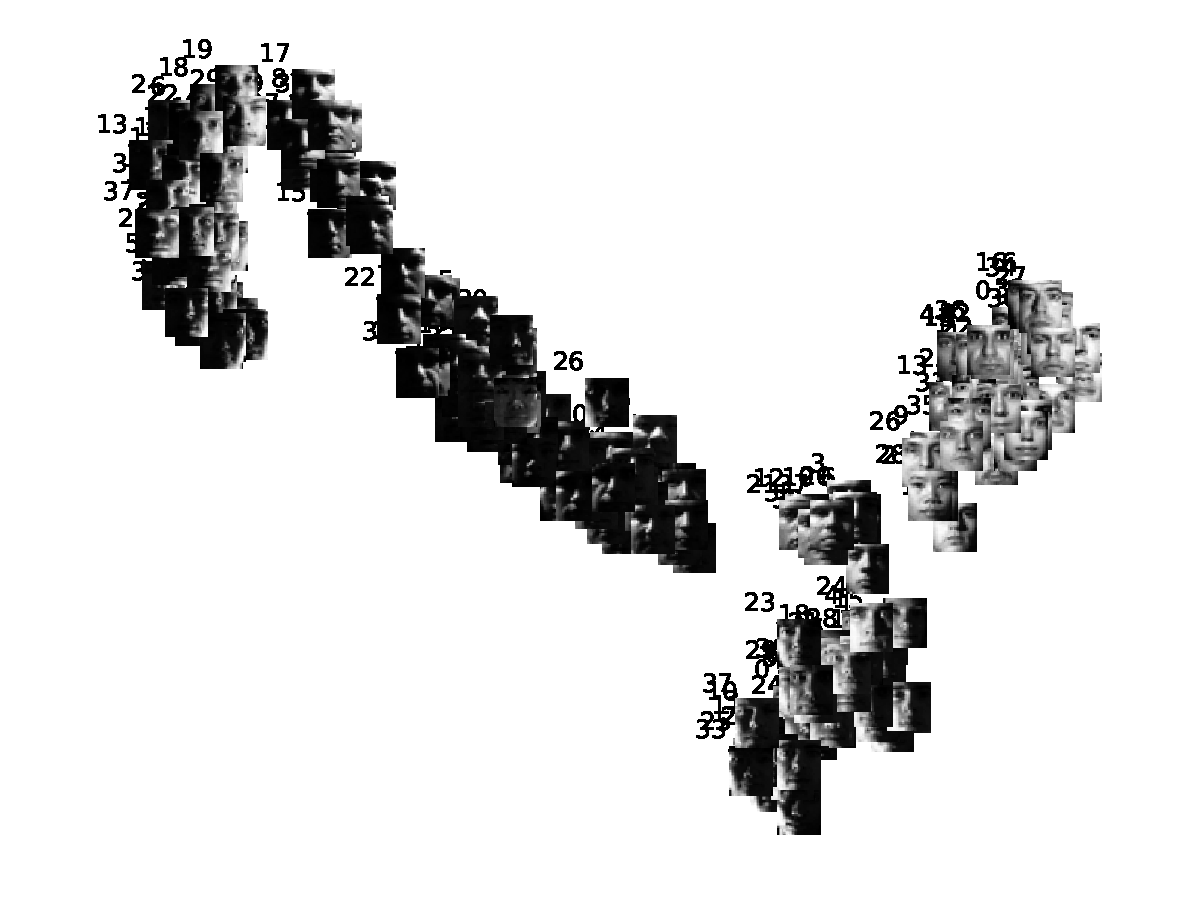
\includegraphics[width=\textwidth]{yaleb_x.pdf}
        \caption{}
        \label{fig:yaleb_x}
  \end{subfigure} %
    \begin{subfigure}{.49\textwidth}
      \centering
        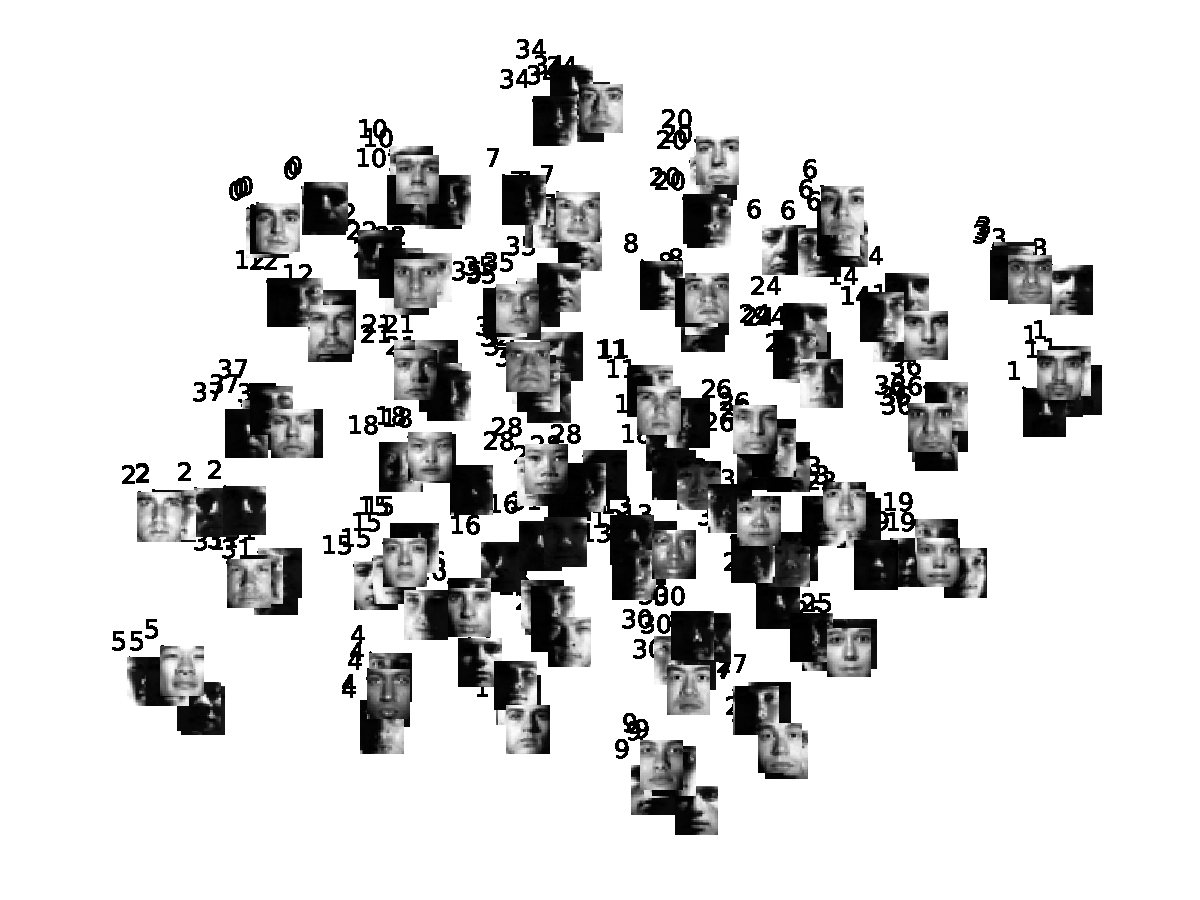
\includegraphics[width=\textwidth]{yaleb_z.pdf}
        \caption{}
        \label{fig:yaleb_z}
     \end{subfigure} % 
    \caption{t-SNE~\citep{2013arXiv1301.3342V} visualizations of the Extended Yale B training set. (a): original $\*x$ , (b):  latent $\*z_1$  from VFAE. Each example is plotted with the person ID and the image. Zoom in to see details.}
    \label{fig:yaleb_via}
\end{figure}
